\chapter{Uncertainty in atomic force predictions}
\label{chapter3}

The reliability of machine-learned interatomic potentials depends not only on the accuracy of reproducing reference quantum mechanical data but also on the ability of such models to quantify uncertainty in predictions, as the desired applications of such ML models are for (large) systems that ground-truth data is inaccessible due to prohibitive scaling and the limits of computational efficiency.
Ensemble-based methods, such as ANI models, offer an empirical approach to assessing predictive confidence; however, a robust, universally applicable, and physically meaningful uncertainty measure for atoms of different species remains a challenge.
In the broader field of deep learning, uncertainty quantification has been explored through various strategies, including ensemble averaging \cite{optimal_ensemble_averaging_naftaly, ensemble_deep_learning_review_ganaie}, scalable uncertainty estimation methods \cite{scalable_uncertainty_scalia, scalable_uncertainty_lakshminarayanan}, and dropout-based implementations \cite{dropout1, dropout2, uncertainty_quantification_dropout_wen} to improve predictive capabilities by temporarily removing nodes from the input and hidden layers. 

These approaches aim to distinguish between epistemic uncertainty, which arises from model limitations and can be reduced with additional training data, and aleatoric uncertainty, which reflects inherent noise in the data itself. 
In atomistic simulations, these principles suggest that uncertainty estimation must capture both model limitations and physical constraints imposed by molecular interactions \cite{uncertainty_atomistic_ml_peterson}.
Within the domain of neural network potentials, ensembles have been widely used to quantify predictive confidence, offering a direct measure of variance in model outputs \cite{uncertainty_of_nnp_ensembles_kahle}. 
However, most existing uncertainty estimation techniques focus on energy predictions, rather than on the fundamental physical quantities that dictate molecular behavior. 
Since forces define the curvature of the potential energy surface, an uncertainty measure derived from force predictions would provide deeper insight into model reliability and transferability.

This chapter explores uncertainty estimation in ANI models without altering the already well-performing neural network model architecture. 
We seek an explainable \cite{uncertainty_quantification_yang} uncertainty quantification metric to determine whether force-based uncertainty offers a more practical and scalable alternative to traditional energy-based uncertainty measures.


\section{Potential Solution for an Atomistic QBC Measure}
\label{sec:uncertainty_potential_solution}

In the search for a reliable atomistic metric to estimate uncertainty in molecular energy predictions, we face a fundamental challenge: the true energy of a system is unknown during inference, making direct error quantification impossible. 
Instead, we require a proxy quantity, one that can be predicted by the network and used as an internal measure of confidence without explicit reference to a ground truth.
Atomic energies, while conceptually appealing, proved unsuitable for this purpose; due to the model-dependent energy decomposition, different networks in the ANI ensemble learn distinct atomic energy contributions, leading to inconsistent assignments across models.
Attempts to reduce the uncertainty in predicted atomic energies in a purely data-driven ML model inevitably compromises the accuracy of the total molecular energy prediction.

For an uncertainty measure to be viable, it must be supported by fundamental physical principles and computed in an explainable manner within the existing neural network framework. 
Unlike atomic energies, forces are directly governed by quantum mechanical principles, as they correspond to the gradient of the potential energy surface with respect to atomic coordinates (Eqn. \ref{eq:force_dE}). 
Because every atom in a molecular system experiences forces, this quantity is universally defined---except in the case of a true global minimum, which is inconsequential for MD applications---offering a more consistent target for uncertainty estimation.

A considered alternative approach could involve using dipole moments as an uncertainty metric, given their sensitivity to electronic structure and molecular geometry.
However, dipoles present two key limitations: they do not exist for certain molecular systems, such as nonpolar molecules, and they are global properties, meaning they do not offer localized atomic-level uncertainty estimates.
In contrast, atomic forces remain well-defined even in near-equilibrium geometries, with only minor fluctuations in magnitude depending on molecular stability.

Since molecular dynamics simulations almost exclusively explore non-equilibrium conformations, the forces acting on atoms are virtually always nonzero, reinforcing their utility as a generalizable measure of model confidence.
Even in the case of global equilibrium, models should be tuned to agree on atomic forces predicted to be equal to zero. 
Thus, forces present a promising avenue for quantifying predictive uncertainty at the atomistic level and can be used to explore whether the variability in these values provides a meaningful, physically grounded measure of model reliability.


\subsection{Force Directional Predictions}
\label{subsec:forces}

Atomic forces provide a direct means of assessing the landscape of the potential energy surface (PES), making them a natural candidate for evaluating uncertainty in ANI predictions. 
Since forces correspond to the gradient of energy with respect to atomic positions, they encode local curvature information that is critical for modeling molecular behavior, including geometry optimizations, vibrational properties, and molecular dynamics simulations. 
Unlike atomic energy decompositions, which lack a strict physical interpretation, atomic forces are observable, well-defined, and physically meaningful across all molecular systems.

Forces act on individual atoms and directly govern how they respond to their immediate chemical environment. This atom-wise resolution makes forces particularly valuable for assessing model performance at a finer scale, where uncertainty can be linked to specific atomic interactions rather than a global molecular quantity. 
Because forces inherently reflect the steepness and shape of the potential energy surface, they provide insight into how well the model captures subtle variations in bonding, steric effects, and reaction coordinates that highlight the importance of accuracy in interatomic potentials.

The first approach taken in assessing model agreement in predicted forces was to compute the cosine similarity of the force vector predicted, for each atom, by each model in the ensemble. This relationship is given in Equation \ref{eq:cosine_similarity}.

\begin{equation}
\text{cosine similarity} = \frac{\vec{f_1} \cdot \vec{f_2}}{\max(\|\vec{f_1}\|_2 \cdot \|\vec{f_2}\|_2, \epsilon)}
\label{eq:cosine_similarity}
\end{equation}

Here, two force vectors, $\vec{f_1}$ and $\vec{f_2}$, which point in exactly the same direction would have a cosine similarity of 1, orthogonal vectors would have a value of 0, and anti-parallel vectors would have a similarity value of -1.
The parameter $\epsilon$ is a small number ($10^{-8}$) to prevent the possibility of division by zero. 
Figure \ref{fig:2d_2xr_comp6v1-forces-cos_sim} presents a per-model cosine similarity analysis of atomic force predictions from COMP6V1 benchmark dataset ($N_\text{atoms}=$ 2,608,858) across the ANI-2xr ensemble compared to reference DFT forces. 

\begin{figure}[H]
    \centering
    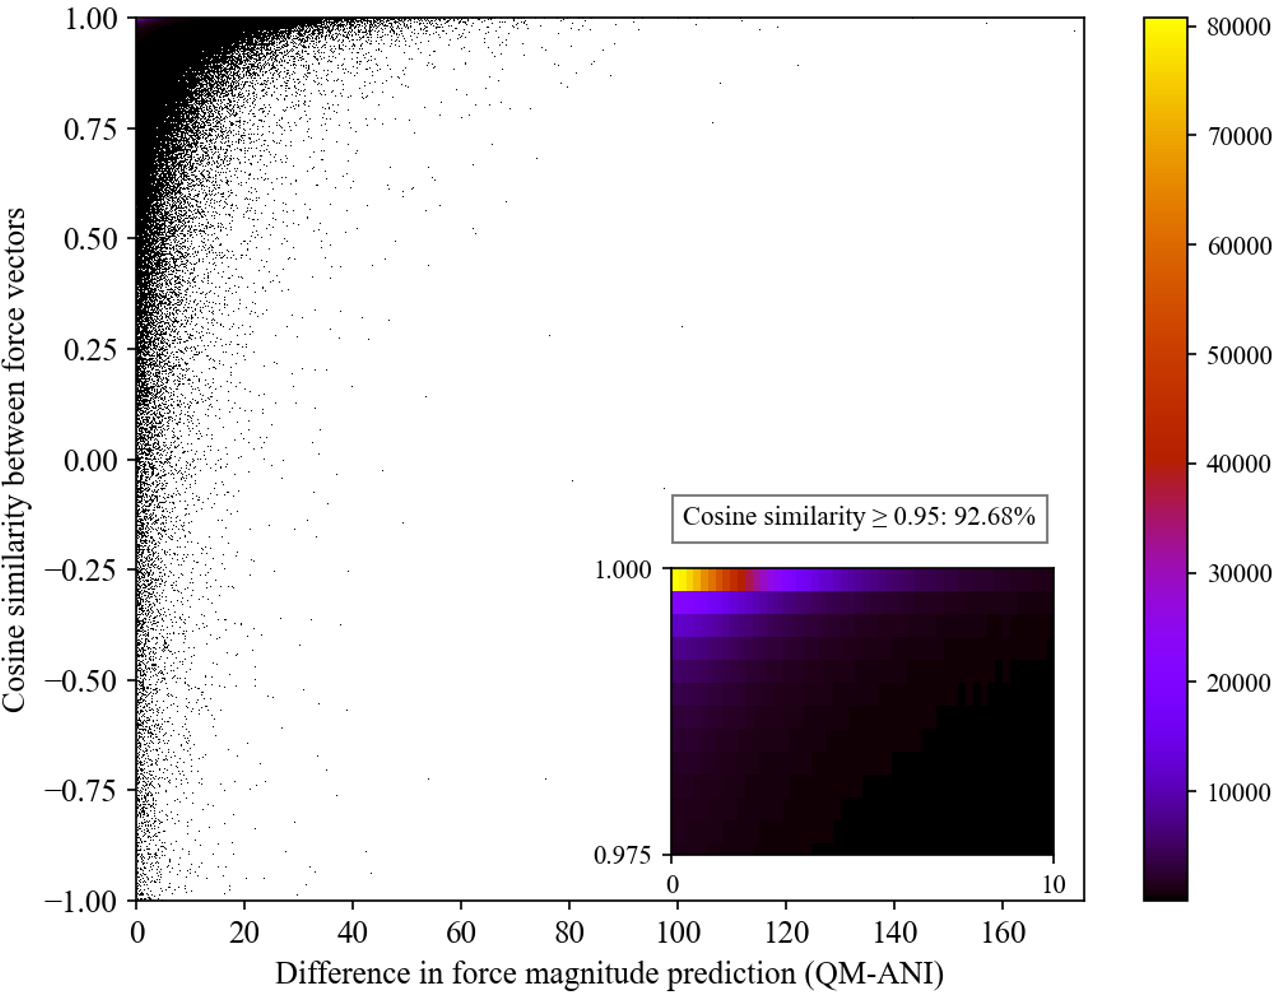
\includegraphics[width=1\linewidth]{Images/2xr_forces/cos_sim-hist2d-insert.png}
    \caption[2D histogram of cosine similarity measure of predicted atomic force vectors]{
    Cosine similarity measure between ANI predicted forces (per-model) versus the DFT reference forces on the COMP6v1 benchmark dataset.
    }
    \label{fig:2d_2xr_comp6v1-forces-cos_sim}
\end{figure}

This metric captures the directional agreement between predicted and true force vectors, illustrating that ANI models, in nearly all cases, predict forces that align closely with the correct direction on the PES. 
Even in cases where predictions deviate, these errors tend to occur in low-error structures near equilibrium, where the magnitude of the force vector is very small. 
This suggests that while absolute force magnitudes vary across the ensemble, the network reliably captures the qualitative features of the PES.
The cosine similarity data is re-plotted in three dimensions in Figure \ref{fig:2xr_comp6v1-forces-cos_sim}, further demonstrating the directional agreement of predicted atomic forces.

\begin{figure}[H]
    \centering
    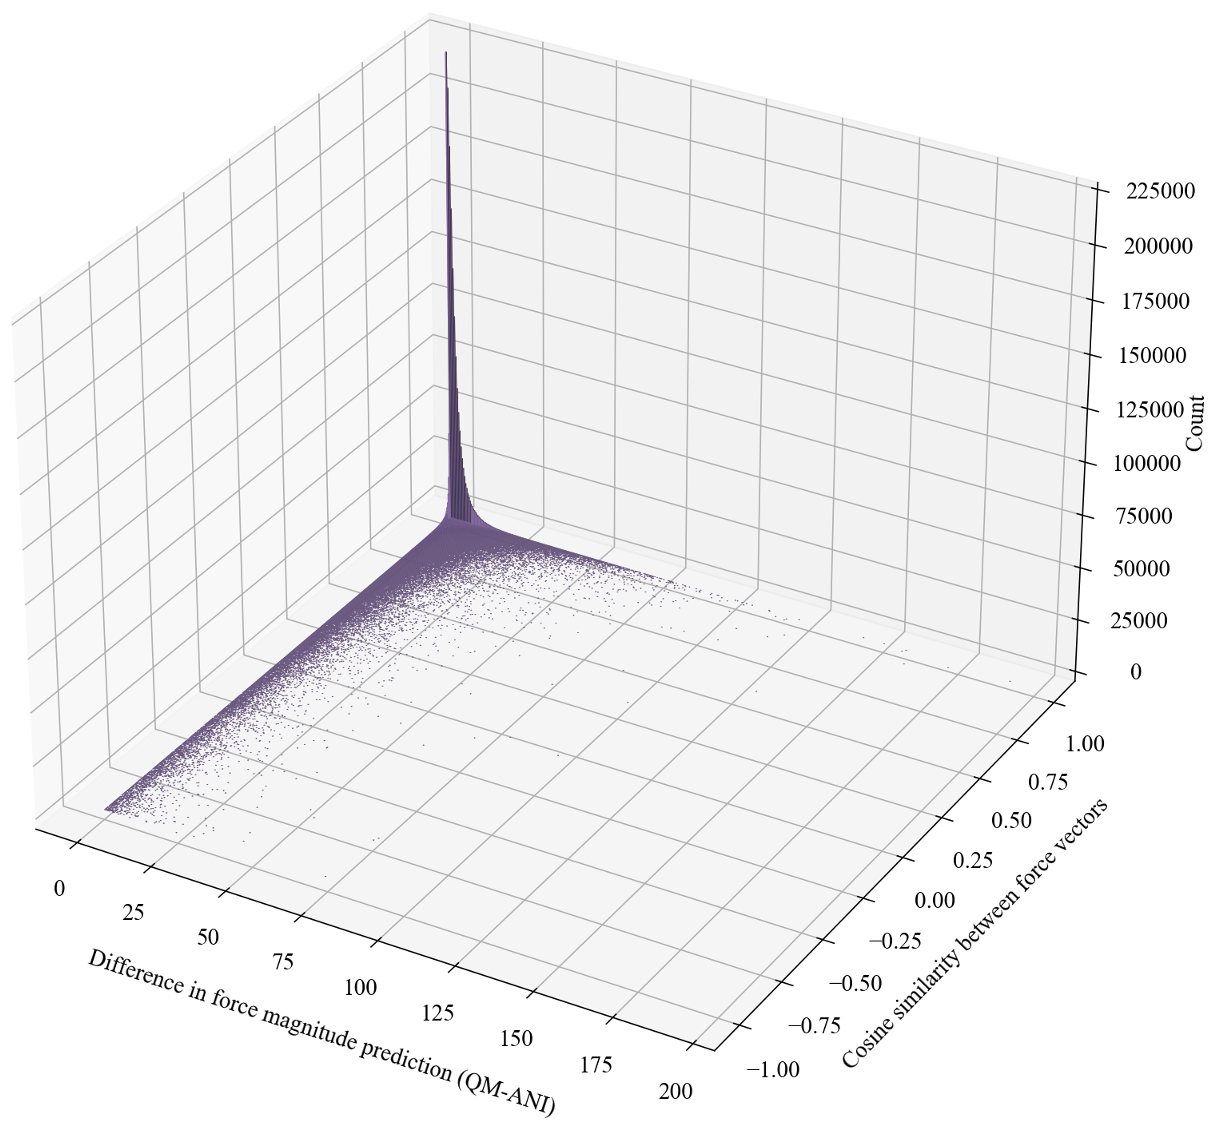
\includegraphics[width=1\linewidth]{Images/2xr_forces/2xr_comp6v1_force-cosine_sim-bar3d.png}
    \caption[3D histogram of cosine similarity measure of predicted atomic force vectors]{
    Cosine similarity measure between ANI predicted forces (per-model) versus the DFT reference forces against force magnitude prediction (kcal/mol*$\angstrom$) on the COMP6v1 benchmark dataset.
    }
    \label{fig:2xr_comp6v1-forces-cos_sim}
\end{figure}


One of the key advantages of using force predictions for uncertainty quantification is their sensitivity to local errors in the PES. 
Atomic forces provide spatially resolved information that reflects the stability of individual atoms within their local chemical environment. 
The strong directional agreement between DFT forces and ANI-predicted forces suggests that, while there is some deviation from the reference forces, the predicted PES captures the energy landscape produced by DFT computations.

Ensemble-based predictions of atomic forces allow for a more granular assessment of uncertainty, where high-uncertainty atoms may indicate regions of the molecule that are poorly represented in the training data. 
In ANI, force vectors are obtained independently from each model within the ensemble, meaning that variations in force predictions across the ensemble provide a direct measure of model disagreement; a high variance in force predictions signals regions of chemical space where the model lacks confidence.
Importantly, unlike atomic energies, which exhibit compensatory behavior across the ensemble (as discussed in Section \ref{sec:uncertainty_atomic_energies}), force predictions sum to a fixed total value of zero. 
This means that force uncertainty is not artificially constrained, making it a more reliable measure of true model uncertainty rather than an artifact of network training.

Beyond uncertainty quantification, force predictions also offer practical advantages for improving the robustness of ANI models. 
Since forces define the shape and curvature of the PES, incorporating force-based uncertainty into active learning strategies could enhance the selection of training data, ensuring that new data points are sampled in regions of highest uncertainty. 
This approach has been explored in other uncertainty-aware machine learning models \cite{uncertainty_atomistic_ml_peterson}, but its application to force-driven active learning in ANI remains an open area of research.
The strong directional agreement between ANI-predicted and reference forces demonstrates that, even in cases of mild uncertainty, the model remains faithful to the underlying physics of molecular interactions.

While atomic forces present a promising avenue for uncertainty quantification, they also introduce a new challenge: each atom's force prediction consists of three independent vector components, corresponding to the $x$,$y$, and $z$ directions. 
Unlike total energy, which is a scalar quantity that can be directly compared across different molecules, force vectors introduce dimensional complexity when attempting to reduce uncertainty to a single measure. 
A meaningful uncertainty metric must distill this multi-component information into a single scalar value that captures the reliability of force predictions without discarding essential physical details.

Force vectors inherently contain two distinct aspects: direction and magnitude. 
In the previous analysis, we evaluated force directionality by considering cosine similarity between predicted and reference force vectors. 
This measure allowed us to assess how well the ANI models capture the qualitative structure of the potential energy surface, ensuring that forces point in the correct directions even when individual model predictions differ. 
However, directional agreement alone does not provide a complete picture of uncertainty; forces with similar orientations may still differ significantly in magnitude.

To develop a comprehensive force-based uncertainty measure, it is necessary to investigate the second aspect of force predictions: magnitude variations across the ensemble. If models in the ensemble consistently predict similar force magnitudes, we can infer that the model is making confident predictions in that region of chemical space. Conversely, if the ensemble exhibits high variance in force magnitudes, this suggests increased uncertainty, potentially indicating that the model has encountered an unfamiliar molecular environment.

The following sections will focus on force magnitude variability as a key metric for uncertainty estimation. 
By examining how force magnitudes fluctuate across the ensemble, we aim to construct a single, physically meaningful uncertainty measure that accounts for both the direction and strength of predicted atomic interactions.

\subsection{Force Magnitude Predictions}
\label{subsec:force_magnitudes}

While the previous section demonstrated that ANI models accurately predict the direction of atomic forces, an equally important aspect of force reliability is their magnitude. 
The magnitude of an atomic force vector determines how strongly an atom is being pulled or pushed within the potential energy surface (PES), making it a crucial factor in molecular dynamics simulations, vibrational analysis, and transition state searches. 
If a neural network potential (NNP) systematically underestimates or overestimates force magnitudes, it could lead to unphysical behavior in applications of the model.
Figure \ref{fig:2xr_comp6v1-forces-ani_vs_ref} presents a comparison between the mean force magnitudes predicted by ANI-2xr model and the corresponding reference DFT forces across every atom in the COMP6v1 benchmark dataset. 

\begin{figure}[H]
    \centering
    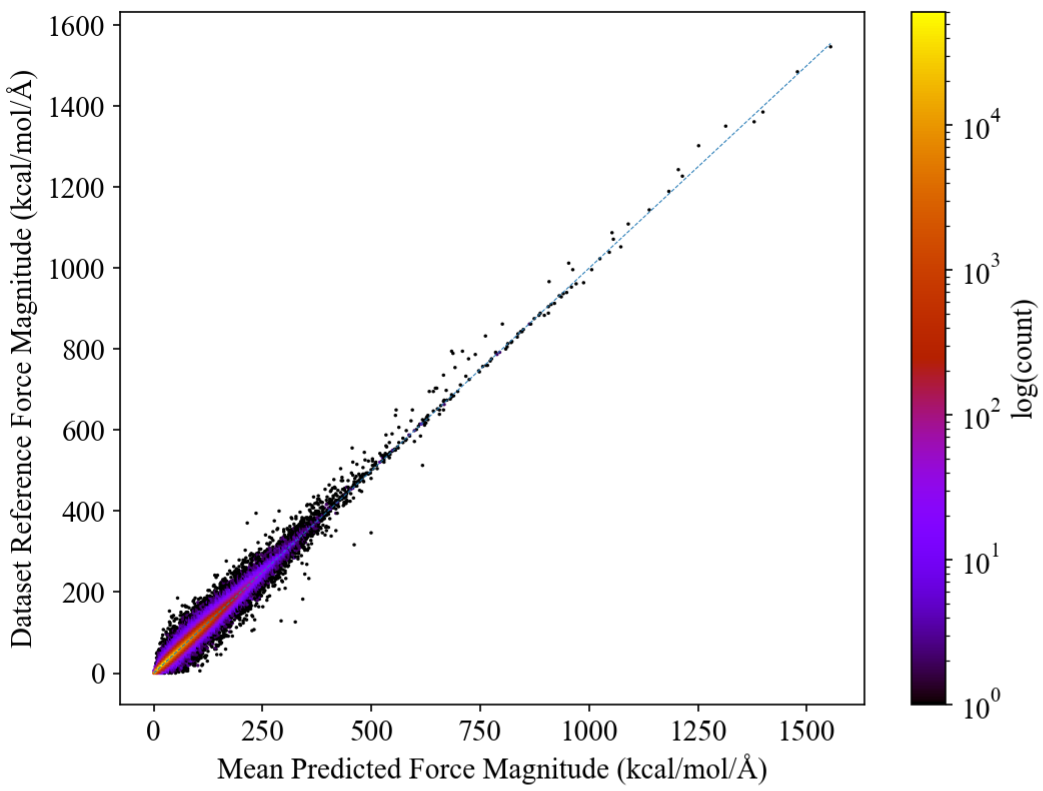
\includegraphics[width=1\linewidth]{Images/2xr_forces/2xr_comp6v1_force-dft-vs-mean_ani.png}
    \caption[Mean predicted atomic force magnitude versus DFT reference (COMP6v1)]{Predicted force magnitudes versus DFT ($\omega$B97X) reference force magnitudes on the COMP6v1 benchmark dataset ($N_\text{atoms}=$ 2,608,858).}
    \label{fig:2xr_comp6v1-forces-ani_vs_ref}
\end{figure}

The near-perfect correlation indicates that ANI is not only capable of capturing the qualitative structure of the PES (as seen in Figures \ref{fig:2d_2xr_comp6v1-forces-cos_sim} and \ref{fig:2xr_comp6v1-forces-cos_sim}) but also reproduces the quantitative force magnitudes with remarkable accuracy. 
One might question whether force magnitudes could serve as an effective uncertainty measure, given the high-level of accuracy in the mean predicted values: if ANI reliably reproduces DFT-level force magnitudes, does this not suggest that the atomistic uncertainty is already minimized? 
However, the distribution in Figure \ref{fig:2xr_comp6v1-forces-ani_vs_ref} is a bit misleading.
Though most forces are predicted with very high accuracy, a closer view at the values where most forces fall show off the broader width of this distribution.
Figure \ref{fig:2xr_comp6v1-forces-ani_vs_ref-cropped} shows the hexbin distribution of these points, where it is clear that many forces are predicted with errors ranging into the hundreds of kcal/mol*$\angstrom$.

\begin{figure}[H]
    \centering
    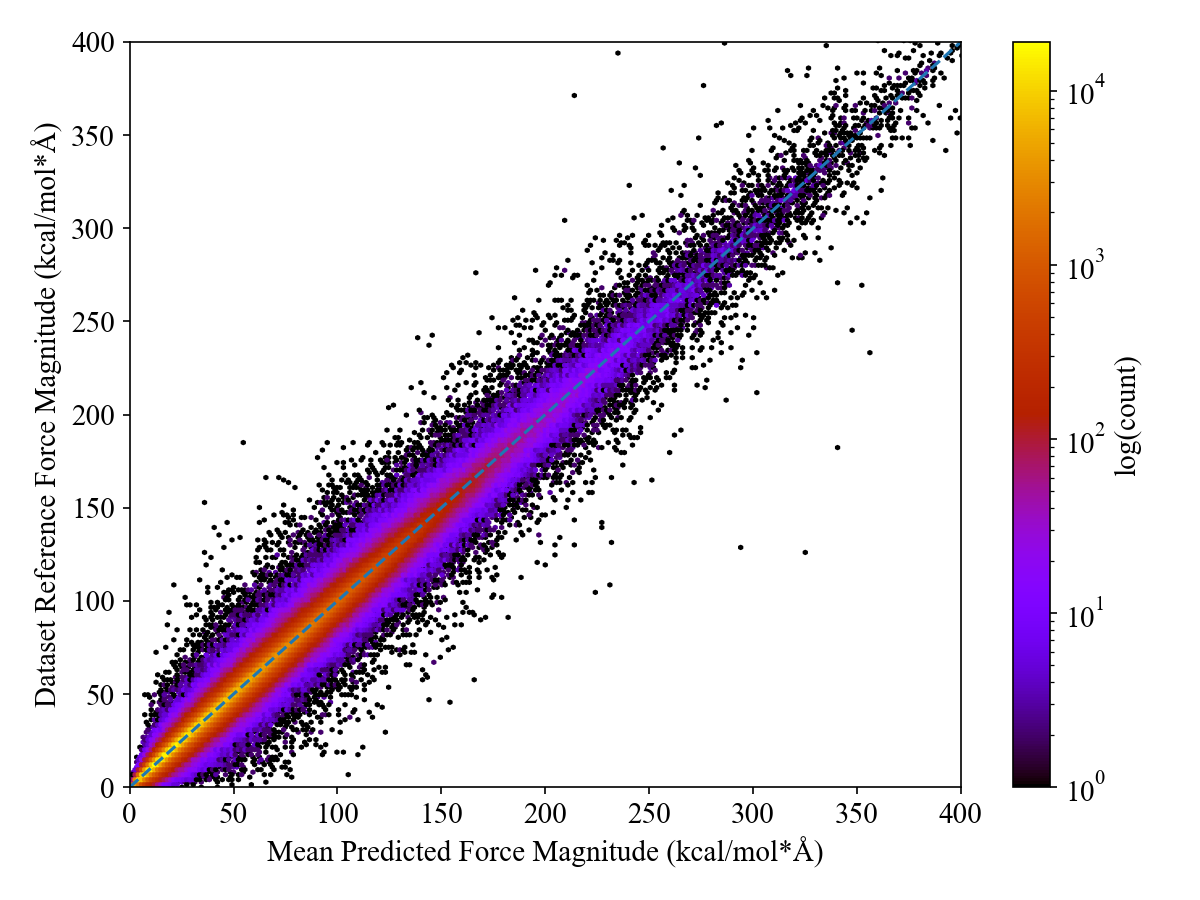
\includegraphics[width=1\linewidth]{Images/2xr_forces/zoomed_2xr_comp6v1_force-dft-vs-mean_ani.png}
    \caption[Cropped atomic force magnitude predictions versus DFT reference (COMP6v1)]{Predicted force magnitudes versus DFT ($\omega$B97X) reference force magnitudes on the COMP6v1 benchmark dataset, cropped at 400 kcal/mol*$\angstrom$ ($N_\text{atoms}=$ 2,608,492).}
    \label{fig:2xr_comp6v1-forces-ani_vs_ref-cropped}
\end{figure}

A strong mean prediction does not necessarily capture error at the atomic level; the figure only represents the mean force magnitudes over all molecules in the dataset, without accounting for per-atom variability or systematic differences among individual models.
While ANI performs well on average, ensemble disagreement may still highlight regions of high-uncertainty, even in cases where the mean force magnitude closely aligns with the DFT reference.

The initial approach to force-based uncertainty quantification was to examine the variance in predicted force magnitudes across the ensemble of ANI models. 
Figure \ref{fig:2xr_comp6v1-forces-stdev} shows the distribution of standard deviation in force magnitude predictions (in kcal/mol*$\angstrom$) across the COMP6v1 benchmark dataset.

\begin{figure}[H]
    \centering
    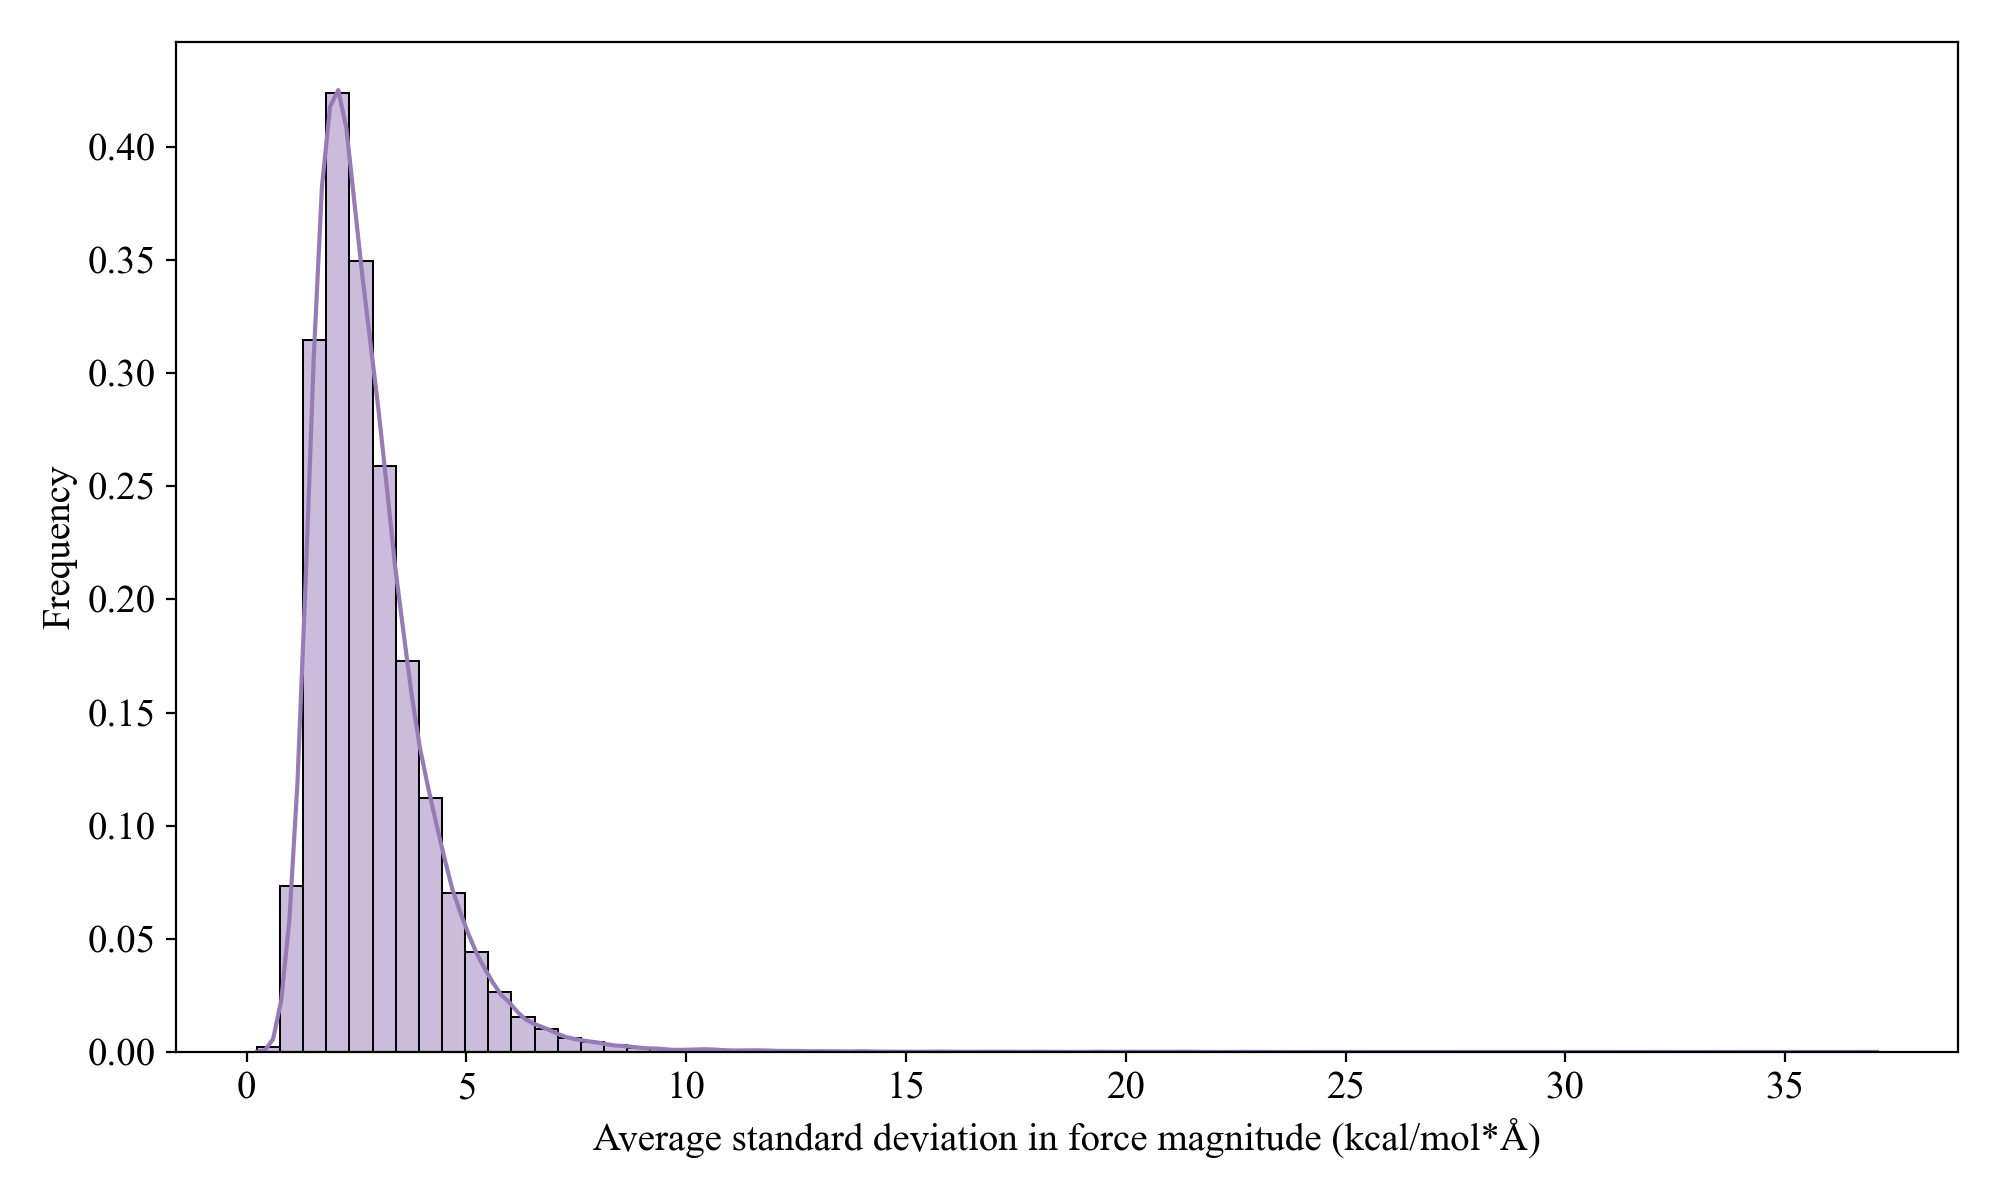
\includegraphics[width=1\linewidth]{Images/2xr_forces/2xr_force_just_stdev.png}
    \caption[Histogram of standard deviation in predicted force magnitudes (COMP6v1)]{Standard deviation in predicted force magnitudes on the COMP6v1 benchmark dataset ($N_\text{atoms}=$ 2,608,858) across the eight-membered ANI-2xr ensemble.}
    \label{fig:2xr_comp6v1-forces-stdev}
\end{figure}

Here, we can see that most forces are determined with a standard deviation ($\sigma$) $\leq 5$ kcal/mol$*\angstrom$, due to the wide range of predicted force magnitudes, as shown in Figure \ref{fig:2xr_comp6v1-forces-ani_vs_ref}.
Some atoms have a very large force magnitude, thus the standard deviation in predictions is inevitably larger than an atom near an equilibrium position.
This makes it difficult to set an exact cutoff after which a force magnitude prediction is untrustworthy, as was done with the energy QBC value by Smith, et al. \cite{ani-1x}.
The size-weighted predictive energy error, normalized by $\sqrt{N_{\text{atoms}}}$, and average standard deviation in predicted force magnitudes per-molecule is given in Figure \ref{fig:2xr_comp6v1-forces-stdev-vs-energy-error}. 
The Pearson correlation coefficient $(\rho_{\text{corr}})$ between these two variables is found to be 0.515.
A linear correlation is not a perfect measure of the correlation between two variables that arise from high-dimensional data.
Rather, we are looking for an uncertainty metric which will relate high-error energy predictions to highly uncertain predictions of some atomistic value.

\begin{figure}[H]
    \centering
    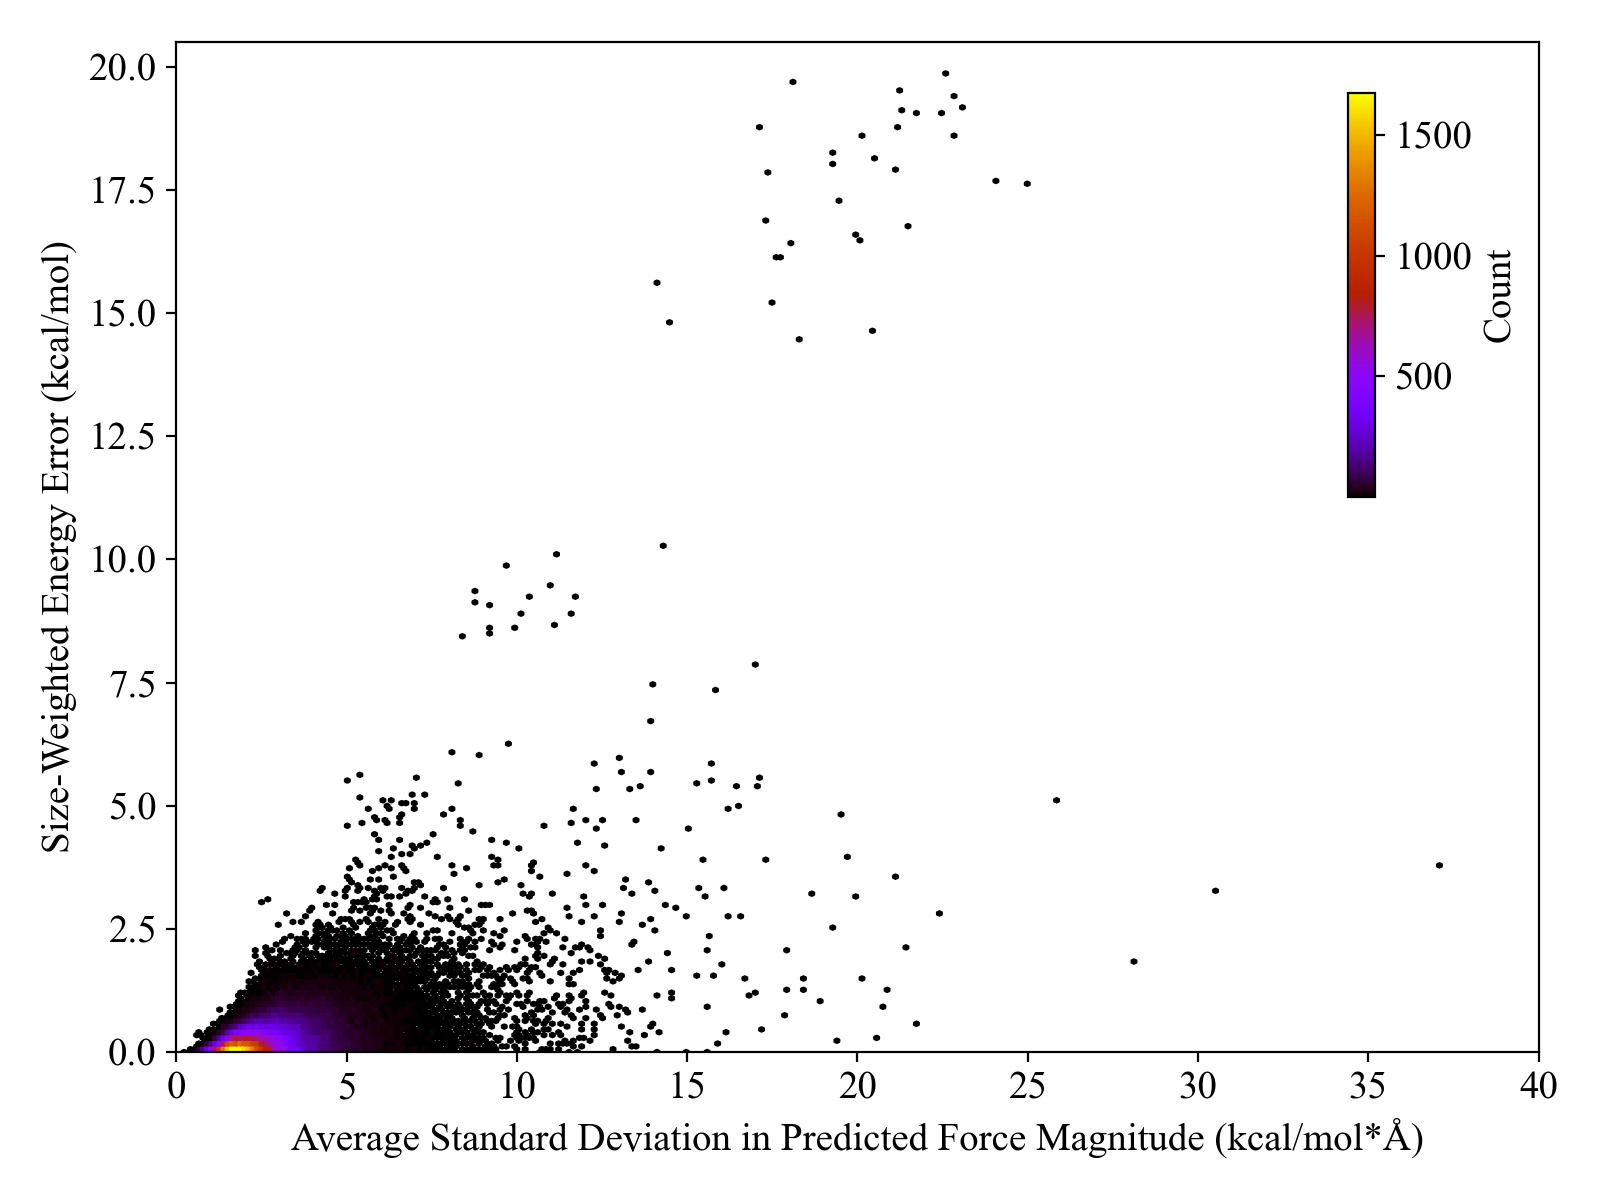
\includegraphics[width=1\linewidth]{Images/2xr_forces/force_stdev-vs-energy_error.png}
    \caption[2D Histogram of standard deviation in predicted force magnitudes versus energy error (COMP6v1)]{Standard deviation in predicted force magnitudes versus size-weighted energy error on the COMP6v1 benchmark dataset  ($N_\text{molecules}=$ 101,352) across the eight-membered ANI-2xr ensemble.}
    \label{fig:2xr_comp6v1-forces-stdev-vs-energy-error}
\end{figure}

While a large average standard deviation in force magnitude does capture the highest-error in energy predictions, setting an exact cutoff on the horizontal axis omits many high-error structures and includes many low-error structures that have a wide range of predicted force magnitudes.
In order to correct for this, many different approaches were considered for normalizing force magnitudes to make them comparable across different atom types and for different scales of force magnitude predictions. 
The following section describes the search for a universally applicable measure of atomistic uncertainty using force magnitude predictions.

\section{Analyzing the Uncertainty of Force Predictions}
\label{sec:analyzing_force_uncertainty}

As force magnitudes depend on both atom type (mass of particle) and the extent to which a structure deviates from equilibrium, direct comparisons across molecules or atomic species can be misleading. 
Ideally, a useful uncertainty measure would highlight high-energy error structures---cases where ANI predictions are unreliable---without being confounded by unrelated factors such as variation in the scale of force magnitudes.
As an initial approach, we examined the standard deviation of force magnitudes across the ANI ensemble (Figures \ref{fig:2xr_comp6v1-forces-stdev} and \ref{fig:2xr_comp6v1-forces-stdev-vs-energy-error}). 
While this metric does capture ensemble disagreement to some extent, it remains heavily biased by the absolute size of the force vectors.
Atoms experiencing large forces tend to have larger standard deviations, even when the model confidence in predicted forces is high. 
To account for this, we next considered the coefficient of variation (relative standard deviation) in Equation \ref{eq:rel_stdev} defined as the standard deviation of force magnitudes divided by the mean force magnitude:

\begin{equation} 
\text{Relative standard deviation} = \frac{\sigma_{|\vec{F}|}}{\mu_{|\vec{F}|}}
\label{eq:rel_stdev}
\end{equation}

This normalization helps to mitigate the absolute magnitude dependence, but still shows strong correlations with vector size. 
Large force magnitudes, even when well-predicted, tend to exhibit higher relative standard deviations, limiting the ability of this metric to consistently identify high-error regions.
As another point of comparison, we introduced an alternative measure: the relative range (Eqn. \ref{eq:rel_range}), which captures the spread of predicted force magnitudes across the ensemble, relative to the mean force magnitude.

\begin{equation} 
\text{Relative range} = 
\frac{\max\limits_{m \in {1, \dots, 8}}\left( |\vec{F}|_m \right) - \min\limits_{m \in {1, \dots, 8}} \left( |\vec{F}|_m \right)}
                            {\mu_{|\vec{F}|}} 
\label{eq:rel_range}
\end{equation}

The scale of these metrics can be seen in the violin plot shown in Figure \ref{fig:2xr_comp6v1-force_uncertainty-violin}.
Ultimately, these approaches perform very similarly to capture the spread of force magnitude predictions.
Visualizing the range of predictions alone is not a useful point of comparison, as we are trying to correlate the uncertainty in force predictions to the error in energy relative to the reference value.

\begin{figure}[H]
    \centering
    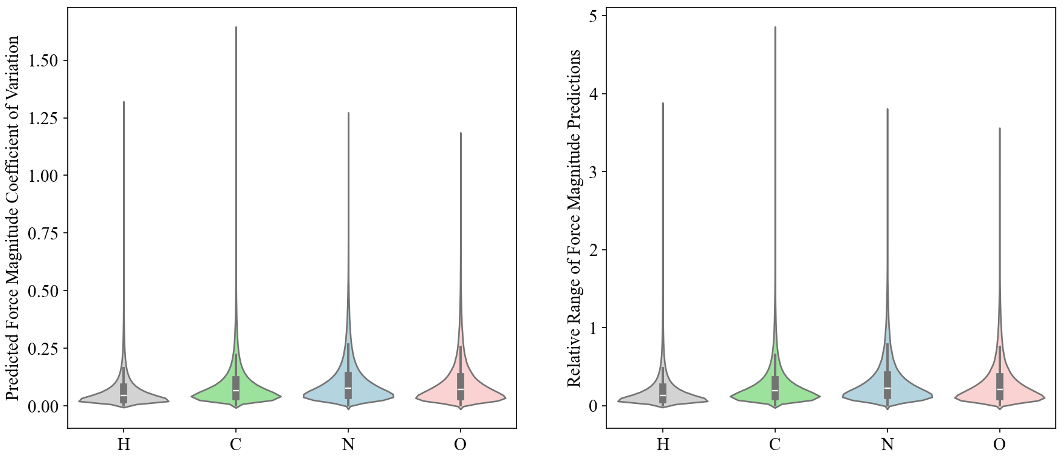
\includegraphics[width=1\linewidth]{Images/2xr_forces/2xr_comp6v1_force-uncertainty_violin.png}
    \caption[Uncertainty in force magnitude predictions: violin distribution (COMP6v1)]{Violin distribution of force magnitude uncertainty measures (relative standard deviation and relative range), computed for ANI-2xr predictions on the COMP6v1 benchmark dataset ($N_\text{molecules}=$ 101,352).}
    \label{fig:2xr_comp6v1-force_uncertainty-violin}
\end{figure}

To determine whether these force-based uncertainty measures provide meaningful insight into ANI model confidence, we must assess their relationship with total molecular energy error. 
Figure \ref{fig:2xr_comp6v1-mean_force_uncertainty_hexbin} presents a direct comparison between these per-molecule averaged force uncertainty measures and size-weighed energy error on the COMP6v1 benchmark dataset. 

\begin{figure}[!ht]
    \centering
    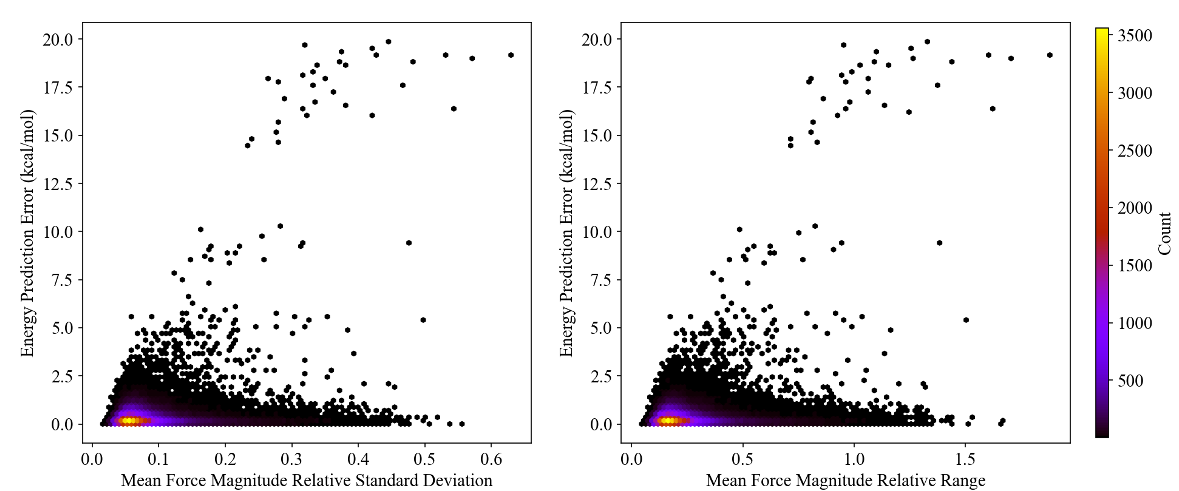
\includegraphics[width=1\linewidth]{Images/2xr_forces/mean-uncertainty-vs-energy.png}
    \caption[Average relative force uncertainty measures per-molecule vs. energy error (COMP6v1)]{Averaged uncertainty measures (relative standard deviation, left; relative range, right) per-molecule on the ANI-2xr predicted forces versus the energy error for the COMP6v1 benchmark dataset ($N_\text{molecules}=$ 101,352).}
    \label{fig:2xr_comp6v1-mean_force_uncertainty_hexbin}
\end{figure}

If a clear correlation is determined, one of these metrics could serve as practical, physics-based uncertainty estimators, enabling more reliable assessments of ANI model reliability without requiring external validation data.
Unfortunately, despite catching extreme outliers, both metrics show a far weaker correlation with the energy prediction error than the QBC.
Averaging either of these values over an entire molecule shows a Pearson correlation coefficient of $\rho_{\text{corr}} \approx 0.09$, while the energy QBC has a $\rho_{\text{corr}} \approx 0.65$ across the COMP6v1 benchmark set.
Further, either metric would lead many structures with low energy errors to be marked as high-uncertainty.
As the average force uncertainty over an entire molecule does not appear to correlate with the error in energy prediction, we aimed to refine our approach further.

Alternative methods of aggregating atomic force uncertainties at the molecular level were investigated. 
We shifted our approach to other measures of spread for the predicted force magnitudes, by looking at the overall spread of force predictions by computing the Mahalanobis distance, $d_\text{M}$, between the ensemble predictions of force magnitudes for each atom $i$, shown in Equation \ref{eq:mahalanobis}.

\begin{equation}
    d_\text{M}\left(\vec{|F|}_i\right) = \sqrt{ \left( \vec{|F|}_i - \mu_{|\vec{F}|_i} \right)^T {\Sigma}^{-1} \left( \vec{|F|}_i - \mu_{|\vec{F}|_i} \right) }
    \label{eq:mahalanobis}
\end{equation}

This produces a measure of spread in predictions for each atom, and we then reduced these to a single value per molecule in two ways: the maximum Mahalanobis distance from any atom within the molecule (Eqn. \ref{eq:max_maha}), and the mean value over the whole molecule (Eqn. \ref{eq:mean_maha}).

\begin{equation}
    d_\text{M}^\text{max} \left(\vec{|F|}\right) = \max_{i \in \{1, \dots, N\}} d_\text{M} \left( \vec{|F|}_i \right)
    \label{eq:max_maha}
\end{equation}

\begin{equation}
    \langle d_\text{M} \left(\vec{|F|}\right) \rangle = \frac{\sum_{i=1}^{N} d_\text{M} \left( \vec{|F|}_i \right)} {N}
    \label{eq:mean_maha}
\end{equation}

Figure \ref{fig:mahalanobis} shows that neither metric captures any correlation between the error in energy prediction and the force magnitudes.
Here, we note that the highest error structures fall around the same maximum or average Mahalanobis distance as the structures with the lowest errors.
Conversely, structures with a large measure of maximum or average Mahalanobis distance tend to have very high accuracy energy predictions.

\begin{figure}[!h]
    \centering
    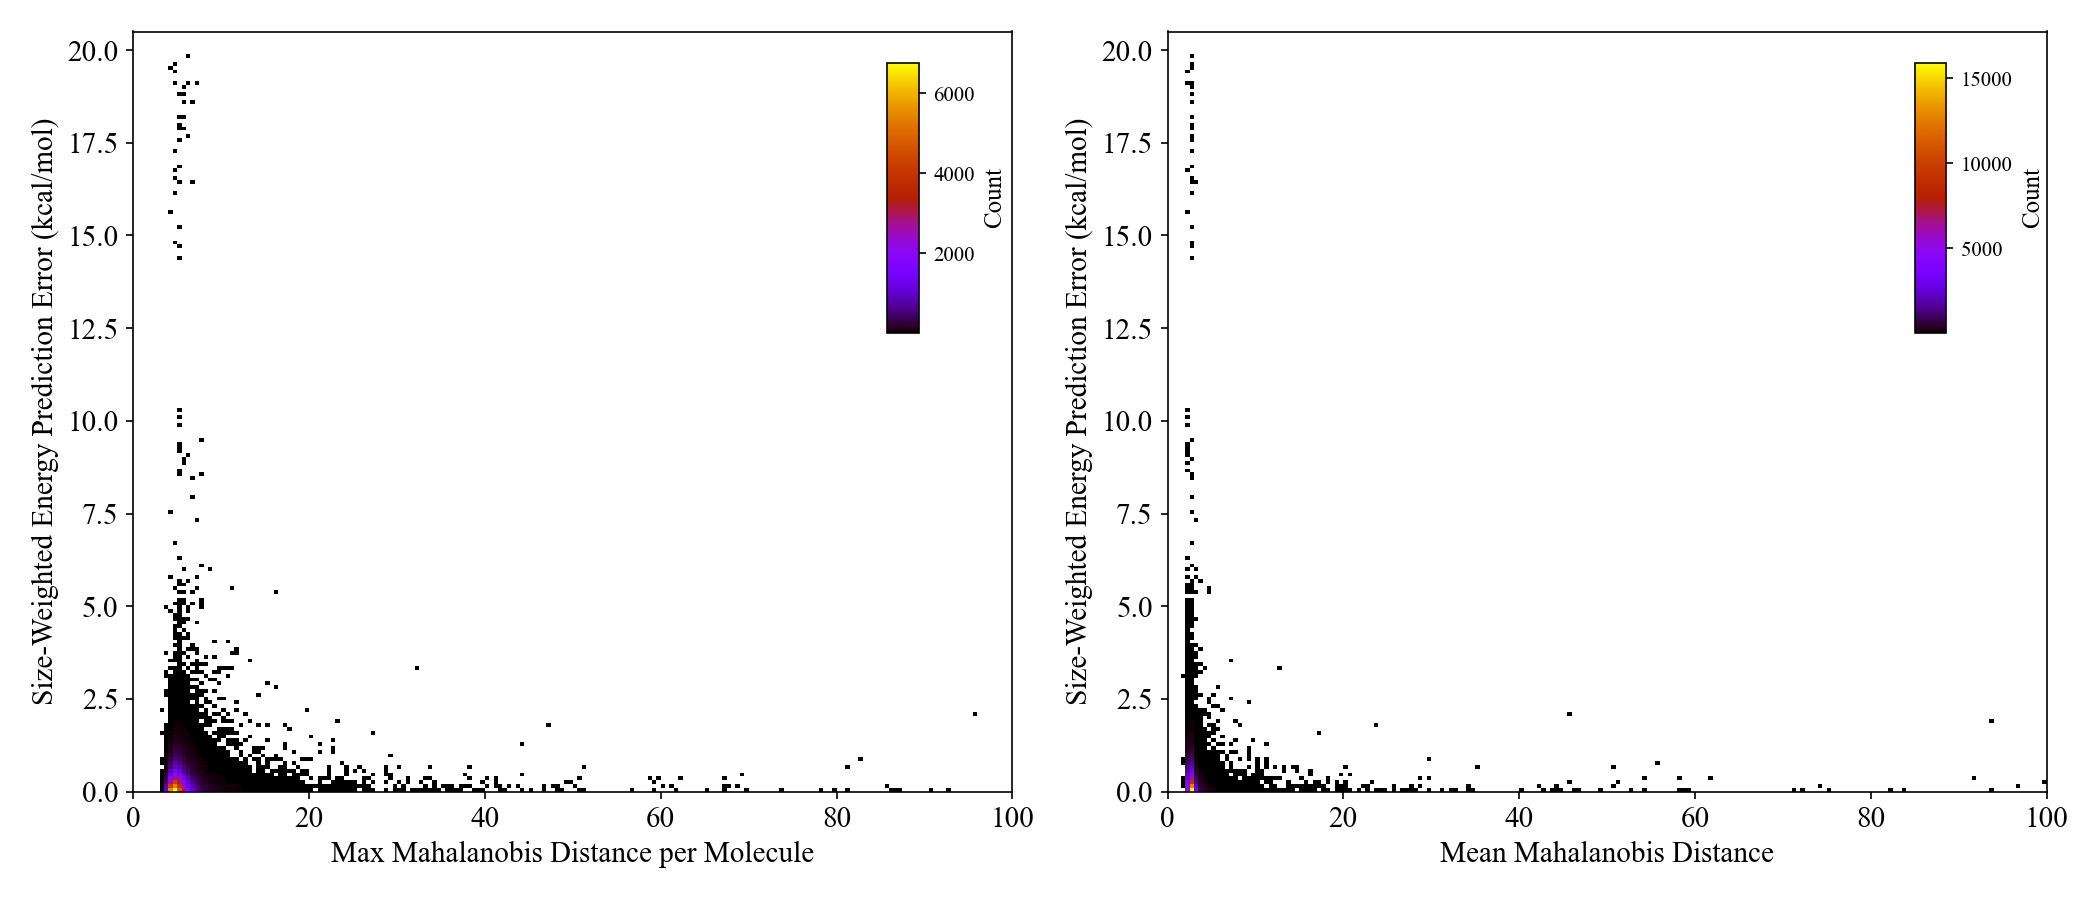
\includegraphics[width=1\linewidth]{Images/2xr_forces/2xr_comp6v1_mahalanobis-uncertainty-vs-energy.png}
    \caption[Mahalanobis distance between ensemble predictions of force magnitude (COMP6v1)]{Maximum Mahalanobis distance between predicted force magnitudes per-molecule (left) and the average Mahalanobis distance over every atom in a molecule (right) plotted against the size-weighted energy error ($N_\text{molecules}=$ 101,352).}
    \label{fig:mahalanobis}
\end{figure}

This suggests that the Mahalanobis distance is not an effective metric for correlating energy error to the predictive spread of force uncertainties, at least when averaging or choosing a single atom as representative of a molecule.
The lack of correlation here shows that, while the Mahalanobis distance measures the spread of force predictions within the ensemble, this spread does not translate directly to errors in total energy prediction.
Further, structures with high values of aggregated Mahalanobis distance do not indicate model failure, but rather that the variations likely arise in high-force regions where the model still performs well.

As a final effort in measuring the spread of force magnitude predictions across the ensemble, we computed the Shannon entropy, $H_{|\vec{F}|_i}$,  for each atom based on the distribution of force magnitudes across the eight ensemble models with Equation \ref{eq:entropy}.

\begin{equation}
    H_{|\vec{F}|_i} = - \sum_{i=1}^{N} \left( \frac{|\vec{F}|_i}{\sum_{j=1}^{N} |\vec{F}|_j} \right) \log \left( \frac{|\vec{F}|_i}{\sum_{j=1}^{N} |\vec{F}|_j} \right)
    \label{eq:entropy}
\end{equation}

As with the Mahalanobis distance, the entropy values were then summarized at the molecular level by computing the maximum (Eqn. \ref{eq:max_entropy}) and the mean (Eqn. \ref{eq:mean_entropy}) entropy values per-molecule. 

\begin{equation}
    H_{|\vec{F}|}^{\max} = \max_{i \in \{1, \dots, N\}} H_{|\vec{F}|_i}
    \label{eq:max_entropy}
\end{equation}

\begin{equation}
    \langle H_{|\vec{F}|} \rangle = \frac{\sum_{i=1}^{N} H_{|\vec{F}|_i}}{N}
    \label{eq:mean_entropy}
\end{equation}

These measures of the distribution of predicted force magnitudes are plotted against the size-weighted energy error in Figure \ref{fig:entropy}.

\begin{figure}[!ht]
    \centering
    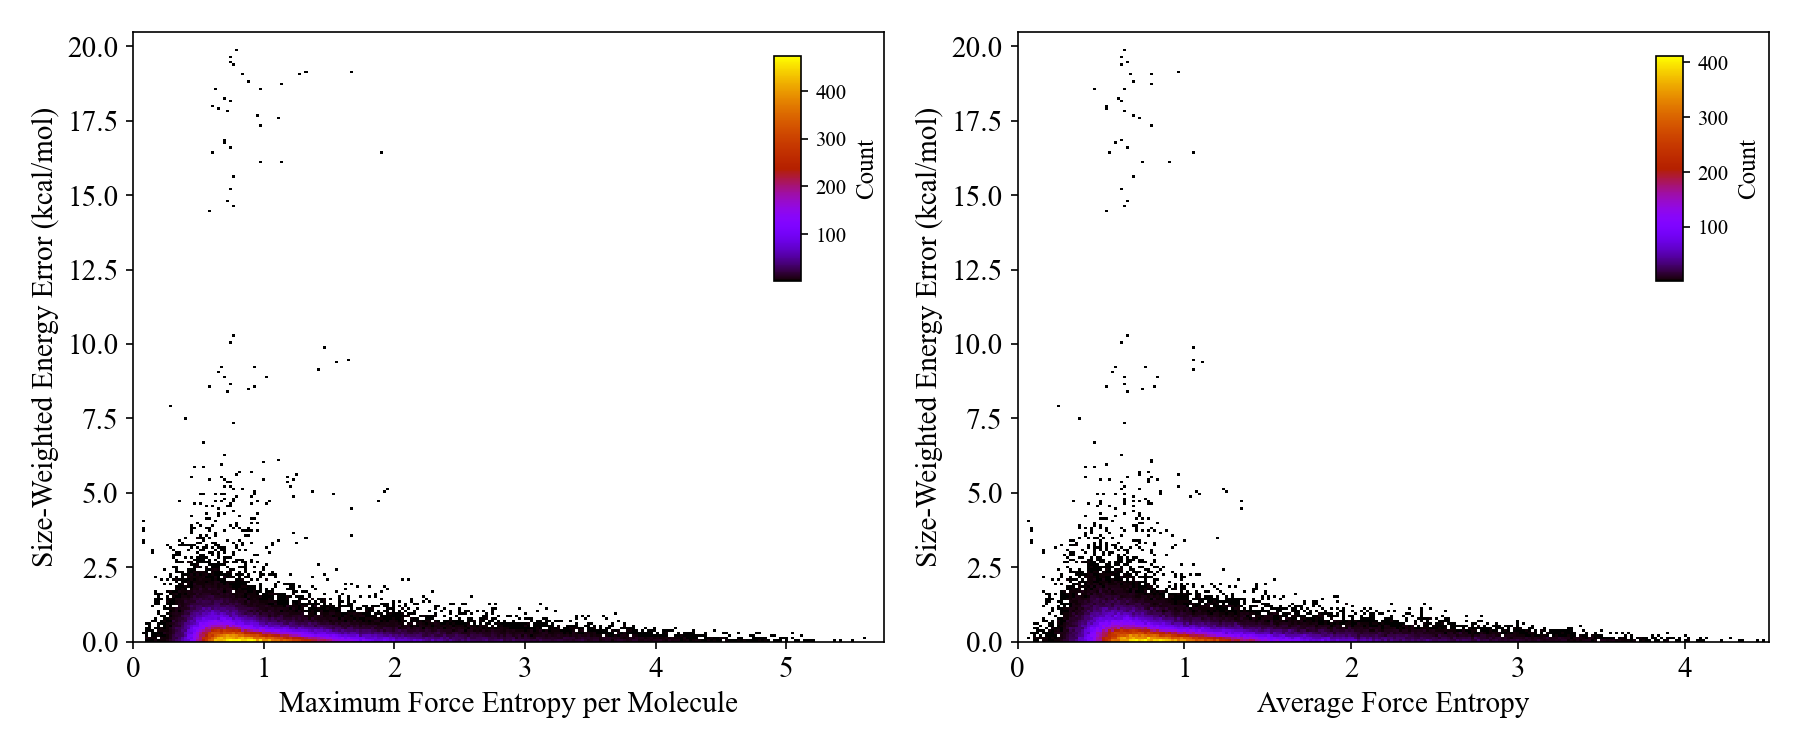
\includegraphics[width=1\linewidth]{Images/2xr_forces/force_entropy-vs-energy.png}
    \caption[Shannon entropy of ensemble predictions of force magnitude (COMP6v1)]{Maximum Shannon entropy between predicted force magnitudes per-molecule (left) and the average entropy over every atom in a molecule (right) plotted against the size-weighted energy error ($N_\text{molecules}=$ 101,352).}
    \label{fig:entropy}
\end{figure}

Large values of entropy would indicate that the spread of predictions for a single atom is very broad and the model cannot agree on the magnitude of a force vector for that atom; small values indicate strong model agreement on force magnitude predictions.
Importantly, while the spread of possible entropy values is much tighter than the Mahalanobis distance measures, the distribution is qualitatively the same as seen in Figure \ref{fig:mahalanobis}.
That is to say, high-error structures have a small maximum or mean entropy value, while the outliers with either entropy measure tend to be structures with low-error energy predictions. 
We note no significant difference between selecting the atom with the highest statistical entropy of predicted force magnitudes and averaging the entropy over an entire molecule. 
In other words, trying to capture the overall spread of predictions and reduce this to a single value per-molecule seems to work against our interest in determining a measure of uncertainty in predicted forces which correlates to the error in energy prediction.

One explanation for this is that energy error arises from a combination of both force magnitude and directional uncertainty, rather than just the spread of force magnitudes alone.
Since relative uncertainties---such as the standard deviation or range of predictions normalized by the mean prediction, as well as the Mahalanobis distance and entropy of per-atom predictions---only consider the variations in force magnitudes, it fails to capture cases where models predict similar magnitudes in different directions.


One possibility was to assign greater importance to highly uncertain atomic forces when computing per-molecule uncertainty scores. 
Figure \ref{fig:2xr_comp6v1-mean_force_uncertainty_hexbin} presents the results of a straightforward averaging approach, where each molecule's force uncertainty is computed as the mean of its atomic uncertainties. 
As this yielded essentially no correlation with molecular energy error, we hypothesized that higher-uncertainty atomic forces might contribute disproportionately to poor energy predictions.
In order to test this, we introduced exponential weighting of atomic force uncertainty measures, increasing the influence of large deviations when computing molecular-level uncertainty. 
The general form of an exponential weighting function used in calculating the weighted mean $u_{\text{weighted}}$ is given in Eqn. \ref{eq:outliers-weighted_sum}, though different weighting parameters were considered.

\begin{equation} 
u_{\text{weighted}} = \frac{\sum_i u_i e^{\alpha w_i}}{\sum_i e^{\alpha w_i}} 
\label{eq:outliers-weighted_sum}
\end{equation}

Here, $u_i$ represents an atomic uncertainty measure (\textit{e.g.}, relative standard deviation or relative range), and $w_i$ is a weighting factor, with an adjustable hyperparameter $\alpha$ controlling the strength of weighting.
The goal was to emphasize large distributions of atomic force predictions, ensuring that molecules with a few highly uncertain atomic forces would be flagged as high-error cases.
The first property considered was the mean cosine similarity, discussed in Subsection \ref{subsec:forces}.
The standard deviation in force magnitude was exponentially weighted by the inverse cosine similarity to compute $u_{\text{weighted}}$, as shown in Equation \ref{eq:force_weighted_cos_sim}.

\begin{equation}
    u_{\text{molecule}} = \frac{\sum_{i=1}^{N} \sigma_{\vec{|F|}_i} \cdot e^{\alpha (1 - \langle \text{cos sim} \rangle_i)}}{\sum_{i=1}^{N} e^{\alpha (1 - \langle \text{cos sim} \rangle_i)}}
    \label{eq:force_weighted_cos_sim}
\end{equation}

Where $\alpha=1$ was the best-performing scaling factor, though we tried $\alpha=0.01, 0.1, 2, 10$, and with each we noted that scaling the by the outliers significantly decreased the efficacy of this approach. 
Each standard deviation in force magnitude $\sigma_{\vec{|F|}_i}$ was weighted by the average cosine similarity $\langle \text{cos sim} \rangle_i$ between ensemble predictions to compensate for force vectors that are predicted with uncertainty in both magnitude and direction.

\begin{figure}[!ht]
    \centering
    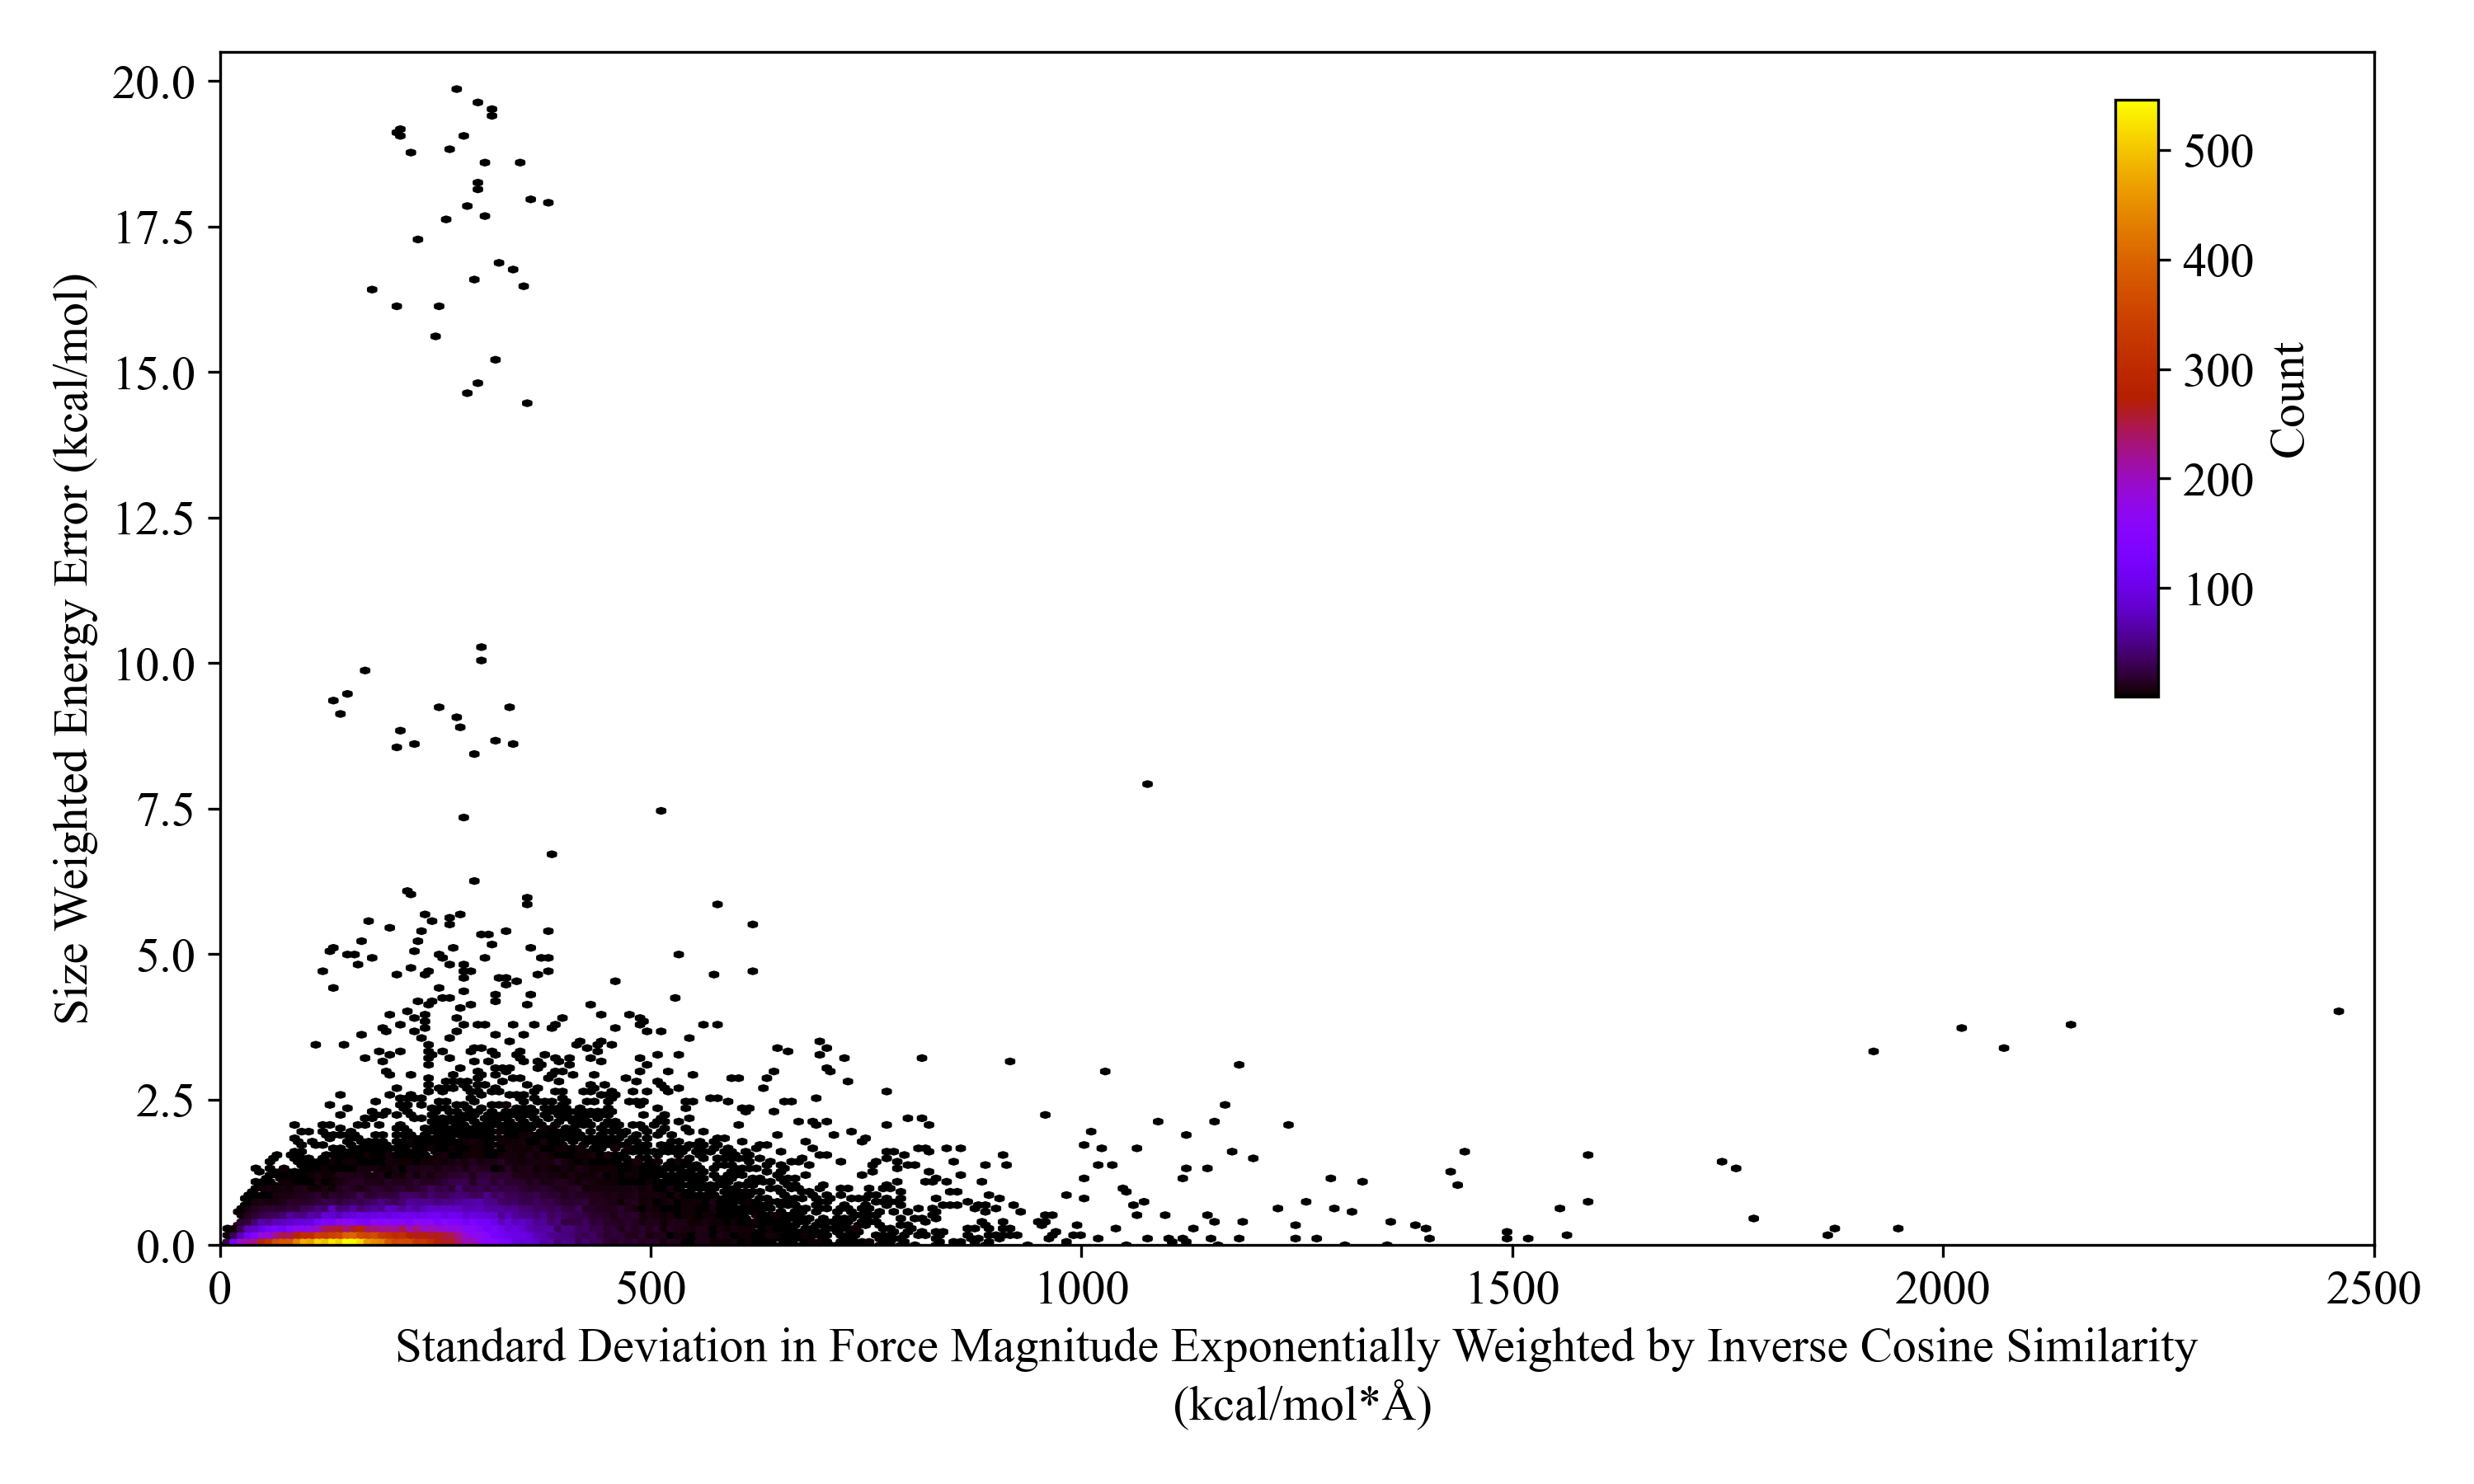
\includegraphics[width=1\linewidth]{Images/2xr_forces/cos_sim_exponential_weighting-vs-energy.png}
    \caption[Standard deviation in force magnitude predictions exponentially weighted by cosine similarity vs. energy error (COMP6v1)]{Standard deviation in force magnitude predictions exponentially weighted by cosine similarity versus size-weighted energy error on the COMP6v1 benchmark dataset ($N_\text{molecules}=$ 101,352).}
    \label{fig:cos_sim-weighted-uncertainty}
\end{figure}

This notably improved the correlation to energy error slightly $(\rho_{\text{corr}}=0.213)$ but clearly does not improve on the trend we are searching to identify, seeing as the worst outliers on the x-axis are far from the highest error structures.
This is not entirely unsurprising, as shown in Figure \ref{fig:2d_2xr_comp6v1-forces-cos_sim}, the force magnitudes with the highest predictive error (relative to DFT forces) have the same directionality as the reference forces.
Deviations in the direction of a force vector tend to be for atoms which are near-equilibrium positions, where the ensemble of models cannot decide which direction would produce a lower-energy structure, while large deviations in magnitude predictions indicate where the ensemble cannot determine how steep the curves of the potential energy surface is (\textit{i.e.}, how far an atom is from an energy minimum).
With that in mind, weighting by the directional outliers puts an undue emphasis on the forces with very small magnitudes.

The next property used in weighting the uncertainty measures was the absolute size of the mean force magnitude prediction, shown in Equation \ref{eq:magnitude-weighted-uncertainty}, where $u_{|\vec{F}|}$ is the uncertainty measure (relative standard deviation or range) for force magnitude prediction and $\mu_{|\vec{F}|_i}$ is the average force magnitude for atom $i$.

\begin{equation}
    \bar{u}_{|\vec{F}|} = \frac{\sum_{i=1}^{N} u_{|\vec{F}|_i} e^{\alpha \mu_{|\vec{F}|_i}}}{\sum_{i=1}^{N} e^{\alpha \mu_{|\vec{F}|_i}}}
    \label{eq:magnitude-weighted-uncertainty}
\end{equation}

Figure \ref{fig:2xr_comp6v1-forces-weighed_uncertainty} shows that this approach performed worse than simply averaging per-atom uncertainties. 

\begin{figure}[H]
    \centering
    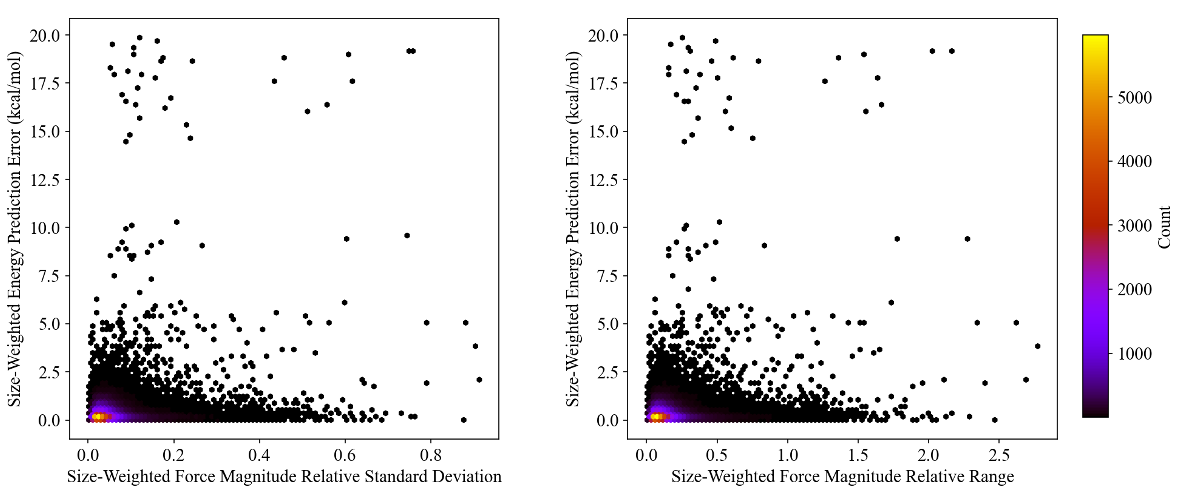
\includegraphics[width=1\linewidth]{Images/2xr_forces/weighted_uncertainty-vs-size_weighted_error.png}
    \caption[Force uncertainty exponentially weighted by outliers versus energy error (COMP6v1)]{Relative standard deviation (left) and range (right) uncertainty measures weighted by outliers in absolute magnitude prediction versus the size-weighted energy error on the COMP6v1 benchmark dataset ($N_\text{molecules}=$ 101,352).}
    \label{fig:2xr_comp6v1-forces-weighed_uncertainty}
\end{figure}

Exponential weighting overemphasizes localized outliers; though the Pearson correlation coefficient remains approximately the same as directly averaging these uncertainty measures $(\rho_{\text{corr}} \approx 0.09)$, we see the visual relationship to molecular energy error has worsened. 

Thus, the search for a force uncertainty metric to correlate with molecular energy prediction error continues.
So far, we have tried averaging relative atom-wise measures, determining outliers in the spread of predictions, and exponentially-weighted averaging of predictive uncertainty, but observe low confidence in these methods to identify high-error structures. 
A new weighting approach was considered: weighting by the sum-total of atomic force magnitudes over an entire molecule.
This provides a similar approach to normalizing by the size of the molecule, adapted for force predictions.
Figure \ref{fig:forces_weighted_by_total_magnitudes} shows this weighting scheme plotted against energy error.

\begin{figure}[!hb]
    \centering
    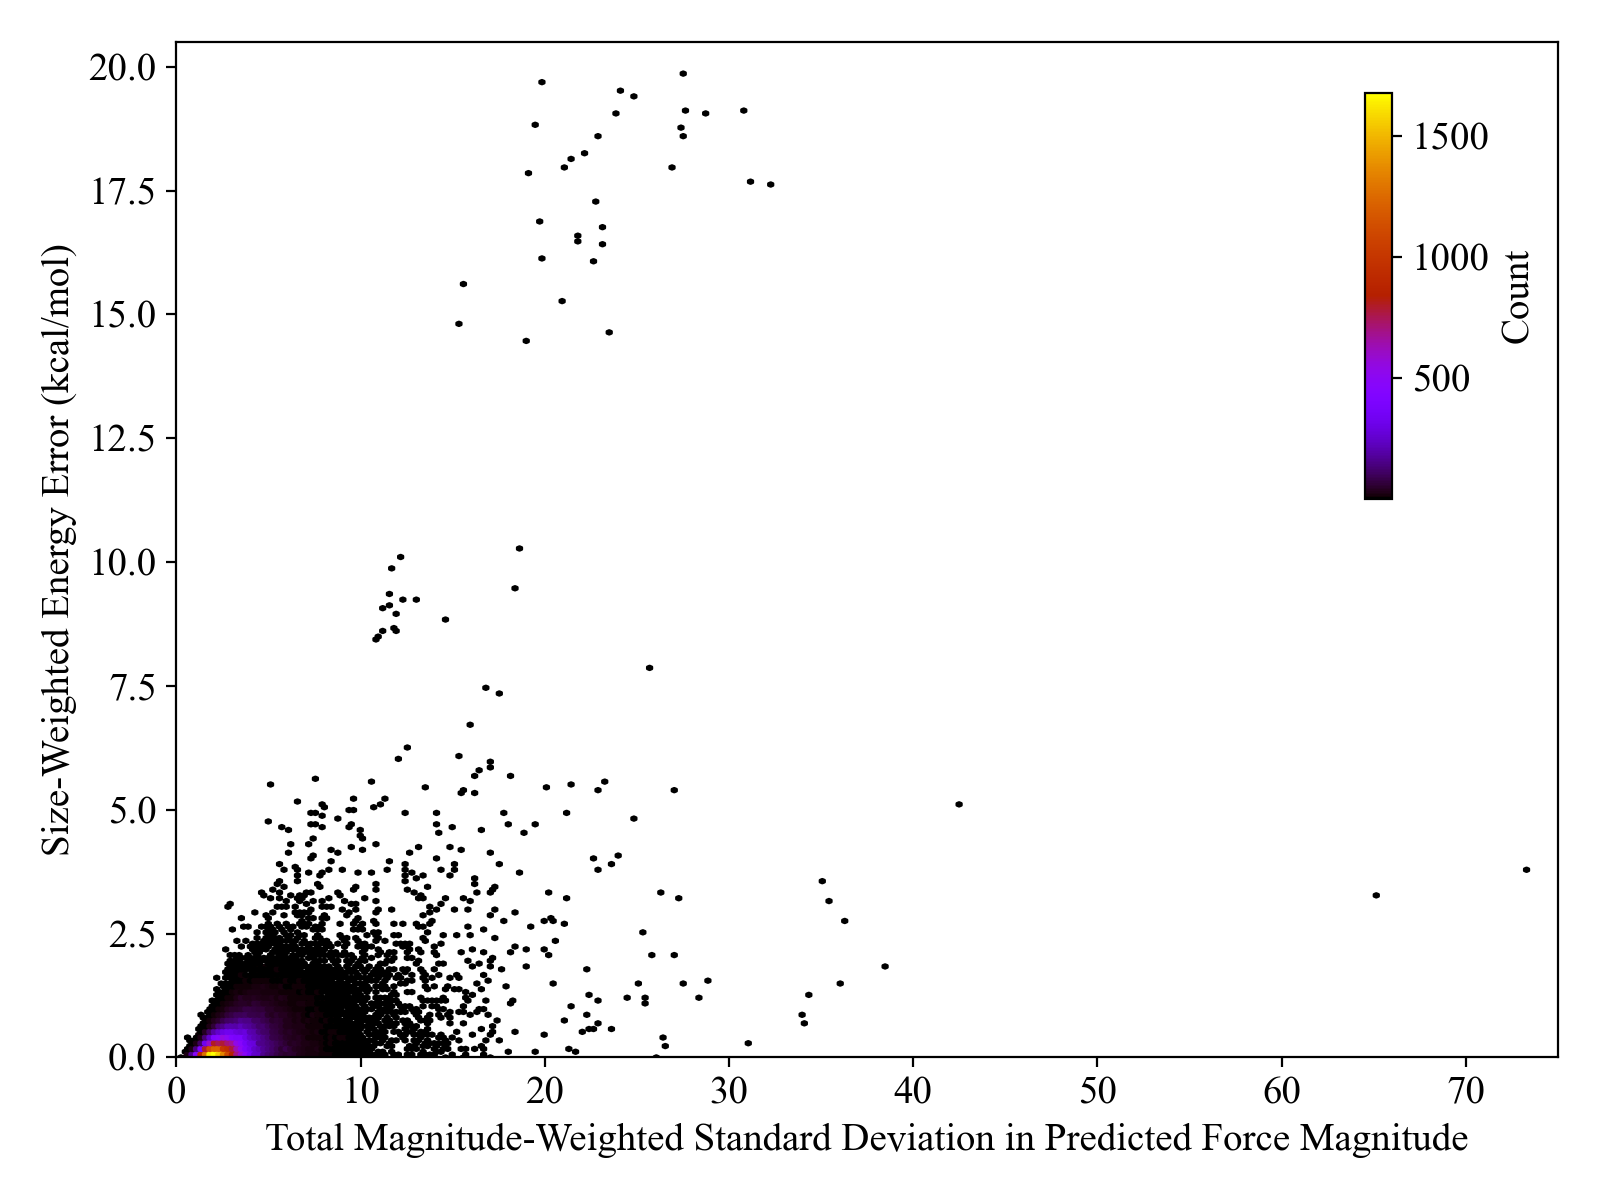
\includegraphics[width=1\linewidth]{Images/2xr_forces/weighted_force_stdev-vs-energy_error.png}
    \caption[Standard deviation of force magnitude prediction weighted by the sum-total of force magnitudes in a molecule (COMP6v1)]{Standard deviation of force magnitude prediction weighted by the sum-total of force magnitudes in a molecule ($N_\text{molecules}=$ 101,352).}
    \label{fig:forces_weighted_by_total_magnitudes}
\end{figure}

We call this measure $\rho_{\vec{|F|}}$, defined in Equation \ref{eq:mag_weighted_force_uncertainty}.

\begin{equation}
    \rho_{\vec{|F|}} = \frac{\sum_{i=1}^{N} \sigma_{|\vec{F}|_i}* \mu_{|\vec{F}|_i}}{\sum_{i=1}^{N} \mu_{|\vec{F}|_i}}
    \label{eq:mag_weighted_force_uncertainty}
\end{equation}

This provided a promising measure of predictive error in molecular energy, with a slightly lower correlation $(\rho_\text{corr} = 0.52)$ than the energy QBC $(\rho_\text{corr} = 0.65)$, but one which is tied to an intrinsically atomistic property.
Unlike previous approaches, this weighting strategy accounts for both the magnitude of atomic forces and their associated uncertainty, providing a more physically meaningful comparison across molecules of different sizes.
This measure captures the intuition that larger total force magnitudes, which are indicative of highly strained systems, should contribute more to the molecular uncertainty measure.
Additionally, this method better distinguishes structures with large energy errors, as molecules with significant force discrepancies contribute disproportionately to energy deviations.

While this metric does not surpass energy QBC in absolute correlation, its direct atomistic connection makes it a more interpretable and transferable uncertainty measure, especially for applications involving molecular dynamics and force-driven reactions.
This is certainly not a perfect measure of force uncertainty, there is room for refinement in this approach by exploring nonlinear scaling factors for weighting, alternative normalization techniques, and comparisons to direct force prediction errors per atom to further bridge the gap between energy uncertainty and force-derived uncertainty measures.
However, it does make clear that there is some way to estimate molecular energy prediction error with the predictive uncertainty of atomic forces.

The ANI-1x paper \cite{ani-1x} states that the QBC value of $\rho = 0.23$ kcal/mol was selected as the value which captures 95\% of the molecular energy errors $\geq 1.5$ kcal/mol.
To translate this measure to the weighted standard deviation, we determine that 95\% of structures with $\Delta E \geq 1.5$ kcal/mol fall above the 
threshold value of $\rho_{\vec{|F|}} \geq 3.5$ kcal/mol*\angstrom. 
This provides a direct mapping between energy-based uncertainty (QBC) and force-based uncertainty, allowing for a more physically meaningful comparison of molecular prediction reliability.
Figure \ref{fig:qbc_vs_energy} shows the relationship between QBC and size-weighted energy error on the COMP6v1 benchmark set, with lines defining $\Delta E = 1.5$ kcal/mol and $\rho_\text{QBC} = 0.23$ kcal/mol.

\begin{flushleft}
\begin{multiFigure}
\centering
    \addFigure{0.75}{Images/2xr_forces/qbc-vs-energy_error.png} \\
    \addFigure{0.75}{Images/2xr_forces/lines_weighted_force_stdev-vs-energy_error.png}
\captionof{figure}[Comparison of energy QBC to force QBC (COMP6v1)]{Comparison of (A) the energy QBC to (B) the weighted standard deviation in force magnitude, both plotted against size-weighted energy error ($N_\text{molecules}=$ 101,352).}
\label{fig:qbc_vs_energy}
\end{multiFigure}
\end{flushleft}

To visualize the data shown in Figure \ref{fig:qbc_vs_energy} more simply, we plot confusion matrices of the values on each quadrant of the dashed red lines in Figure \ref{fig:confusion_matrices} ($N_\text{molecules}=$ 101,352).

\begin{flushleft}
\begin{multiFigure}
\centering
    \addFigure{0.7}{Images/2xr_forces/QBC_confusion.png} \\
    \addFigure{0.7}{Images/2xr_forces/weighted_force_confusion_matrix.png}
\captionof{figure}[Confusion matrices of energy QBC and force QBC (COMP6v1)]{Confusion matrices of (A) the energy QBC ($\rho_\text{QBC}$) to (B) the force magnitude uncertainty ($\rho_{\vec{|F|}}$), both showing predictive energy errors above 1.5 kcal/mol.}
\label{fig:confusion_matrices}
\end{multiFigure}
\end{flushleft}

These confusion matrices visualize which of the structures from the COMP6v1 benchmark set are predicted within the bounds of the $\rho_\text{QBC}$ or $\rho_{\vec{|F|}}$ cutoff for a trustworthy prediction. 
It is important to note here that the new measure for molecular uncertainty, $\rho_{\vec{|F|}}$, captures fewer structures with low error in energy prediction but high uncertainty than the original $\rho_\text{QBC}$-though there are many structures which still fall into this region.
This is valuable for usage in data sampling, as we want a measure which captures the high-error predictions, though these ``false positives" (the yellow, bottom-right quadrants of (A) and (B) in Figure \ref{fig:confusion_matrices}) are inevitable.
While QBC remains the most empirically validated metric for energy error estimation, this force-derived approach highlights the intrinsic connection between atomic force predictions and molecular energy uncertainties. 
Given that forces are derivatives of energy, it is reasonable to expect that discrepancies in force predictions should correspond to discrepancies in energy predictions. 
The challenge, however, lies in identifying per-atom uncertainty which leads to high-error energy predictions.

In order to determine which local atomic environments produce highly-uncertain force predictions, we focused on determining the single largest force deviation per molecule.
This was not expected to be a catch-all metric, as molecules with uncertain force predictions on one atom most likely have uncertain forces on neighboring atoms, but this is a good first approach for determining what a high-uncertainty force prediction is.
The \verb|maximum_deviation| metric is defined in Equation \ref{eq:max_force_deviation}, where $|\vec{F}|_{m_i}$ represents the predicted force magnitude from the $m^{\text{th}}$ model in the ANI ensemble and $\mu_{|\vec{F}|_i}$ represents the mean predicted force magnitude for a given atom across the 8-model ensemble.

\begin{equation} 
\verb|maximum_deviation| = 
\max\limits_{i \in N_{\text{atoms}}}
\frac{\left| \left(\max\limits_{m_i \in {1, \dots, 8}} |\vec{F}|_{m_i} \right)- {\mu_{|\vec{F}|_i}} \right|}{\mu_{|\vec{F}|_i}} 
\label{eq:max_force_deviation}
\end{equation}

The \verb|maximum_deviation| captures the single most extreme disagreement among the ensemble members and selects a single atom as representative of the error per-molecule. 
By normalizing this deviation by the mean force magnitude, this metric prevents small-force predictions (e.g., near equilibrium) from being overshadowed by inherently larger forces, making it a scale-invariant measure of uncertainty.
Figure \ref{fig:2xr_comp6v1-forces-highest_deviation} presents this \verb|maximum_deviation| measure against molecular energy error. 

\begin{figure}[!h]
    \centering
    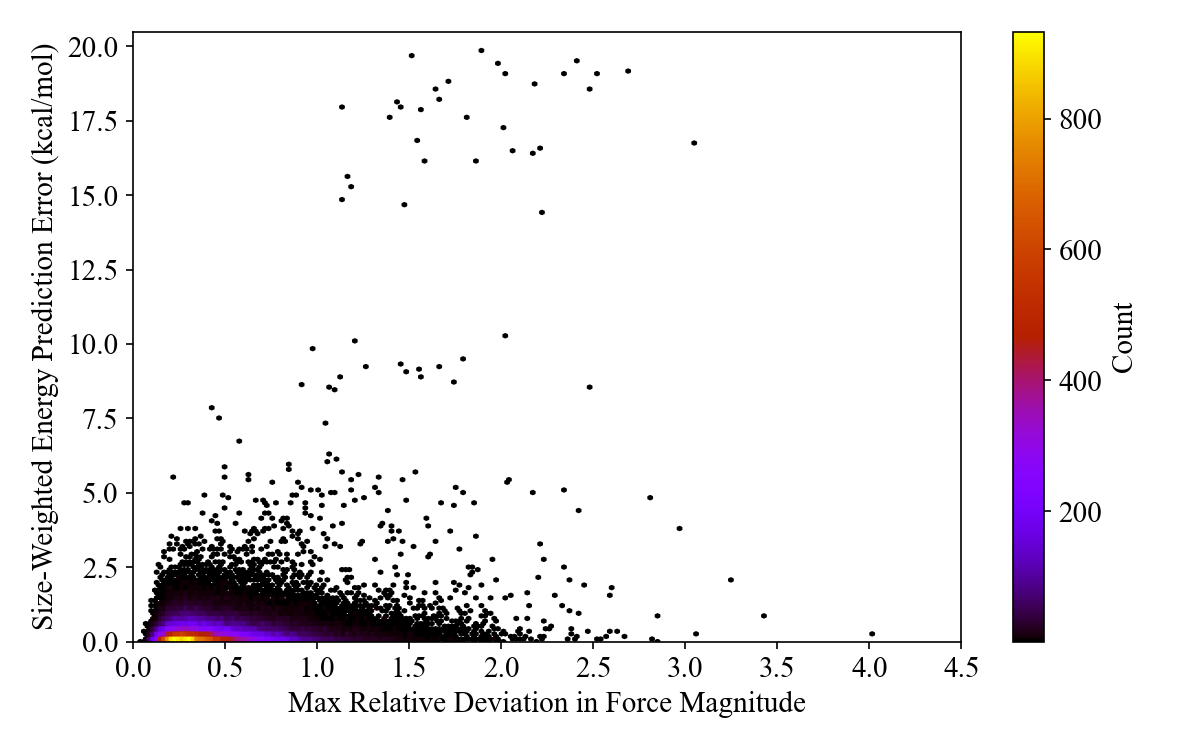
\includegraphics[width=1\linewidth]{Images/2xr_forces/2xr_comp6v1_force-highest-force_deviation-vs-energy.png}
    \caption[Maximum deviation in force magnitude prediction versus energy error (COMP6v1)]{Maximum deviation in force magnitude prediction by ANI-2xr versus energy error on the COMP6v1 benchmark dataset ($N_\text{molecules}=$ 101,352).}
    \label{fig:2xr_comp6v1-forces-highest_deviation}
\end{figure}

The results in Figure \ref{fig:2xr_comp6v1-forces-highest_deviation} demonstrate that \verb|maximum_deviation| in force magnitude prediction serves as a reasonable indicator of the worst-predicted atom in a molecule, but has very low correlation with error molecular energy prediction $(\rho_\text{corr} = 0.122)$.
There could still be utility in this approach: determining which atoms are in local environments which are poorly understood by the ensemble, highlighting regions of the molecule where the model exhibits low confidence. 
This metric could be used to improve the active learning framework: rather than selecting new training data based on the total energy uncertainty of an entire molecular conformation, we can refine the Query by Committee (QBC) process to target high-uncertainty atomic regions.

The original ANI-1x active learning strategy \cite{ani-1x} leveraged energy-based QBC to identify and sample high-uncertainty molecular structures.
The findings presented here suggest a more efficient sampling strategy: instead of selecting entire molecules based on total energy uncertainty, we can prioritize the specific conformations where atomic forces exhibit high model disagreement. 
Applying a data-efficient philosophy to force-based uncertainty could significantly accelerate ANI model training and expand its applicability to larger and more diverse chemical spaces. 
By refining the active learning process to focus on atomic force uncertainty, we could:
(1) Reduce the total amount of required training data while maintaining ANI’s predictive accuracy, similar to the ``less is more" approach demonstrated with ANI-1x. 
(2) Ensure that newly sampled molecules contribute maximally to improving model generalization, by filling in high-uncertainty regions of atomic interactions rather than redundantly adding molecules that contribute little new information. 
(3) Improve transferability to unseen chemical systems by strategically selecting only the conformers that challenge the model, enhancing its ability to generalize beyond its training set.

This would not only reduce computational costs but also enhance the overall accuracy and reliability of ANI predictions, ensuring more consistent performance across a wider range of molecular systems.
Having established that atomic force uncertainty serves as a reliable indicator of molecular energy error, the next logical step is to develop a framework for systematically isolating and refining these high-uncertainty regions. 
We now propose a method to extract and focus on the specific atomic environments that contribute most to uncertainty, which could drastically improve the efficiency of the active learning pipeline.

\subsection{LUKE: Use the Forces}
\label{subsec:luke}

To introduce a more efficient data sampling protocol, we began developing a tool called the Largest Uncertainty Kaleidoscope Estimator: Uncertainty-driven Sampling of high-Error Forces, or LUKE: Use the Forces.
Obviously, we stay within the Skywalker family tree and, being based on the ANAKIN-ME methodology, LUKE is a natural continuation of the ANI approach to data generation.
This tool is designed to automatically identify and extract high-uncertainty atoms from molecular structures. 
The goal of this approach is to refine the active learning process by targeting specific atomic environments rather than entire molecular conformations, thereby improving model accuracy with a smaller, more informative dataset. 
The first step in this process is identifying high-uncertainty atoms. 
Rather than selecting only the highest-uncertainty atom in a system, we use an approach like the \verb|maximum_deviation| in force magnitude prediction, referred to in Equation \ref{eq:atomic_max_force_deviation} as \verb|atomic_deviation|, as an atomistic metric to flag atoms where ensemble disagreement exceeds a given threshold, indicating unreliable model predictions.

\begin{equation} 
\verb|atomic_deviation| = 
\frac{\left| \left(\max\limits_{m_i \in {1, \dots, 8}} |\vec{F}|_{m_i} \right)- {\mu_{|\vec{F}|_i}} \right|}{\mu_{|\vec{F}|_i}} 
\label{eq:atomic_max_force_deviation}
\end{equation}

\begin{figure}[!hb]
    \centering
    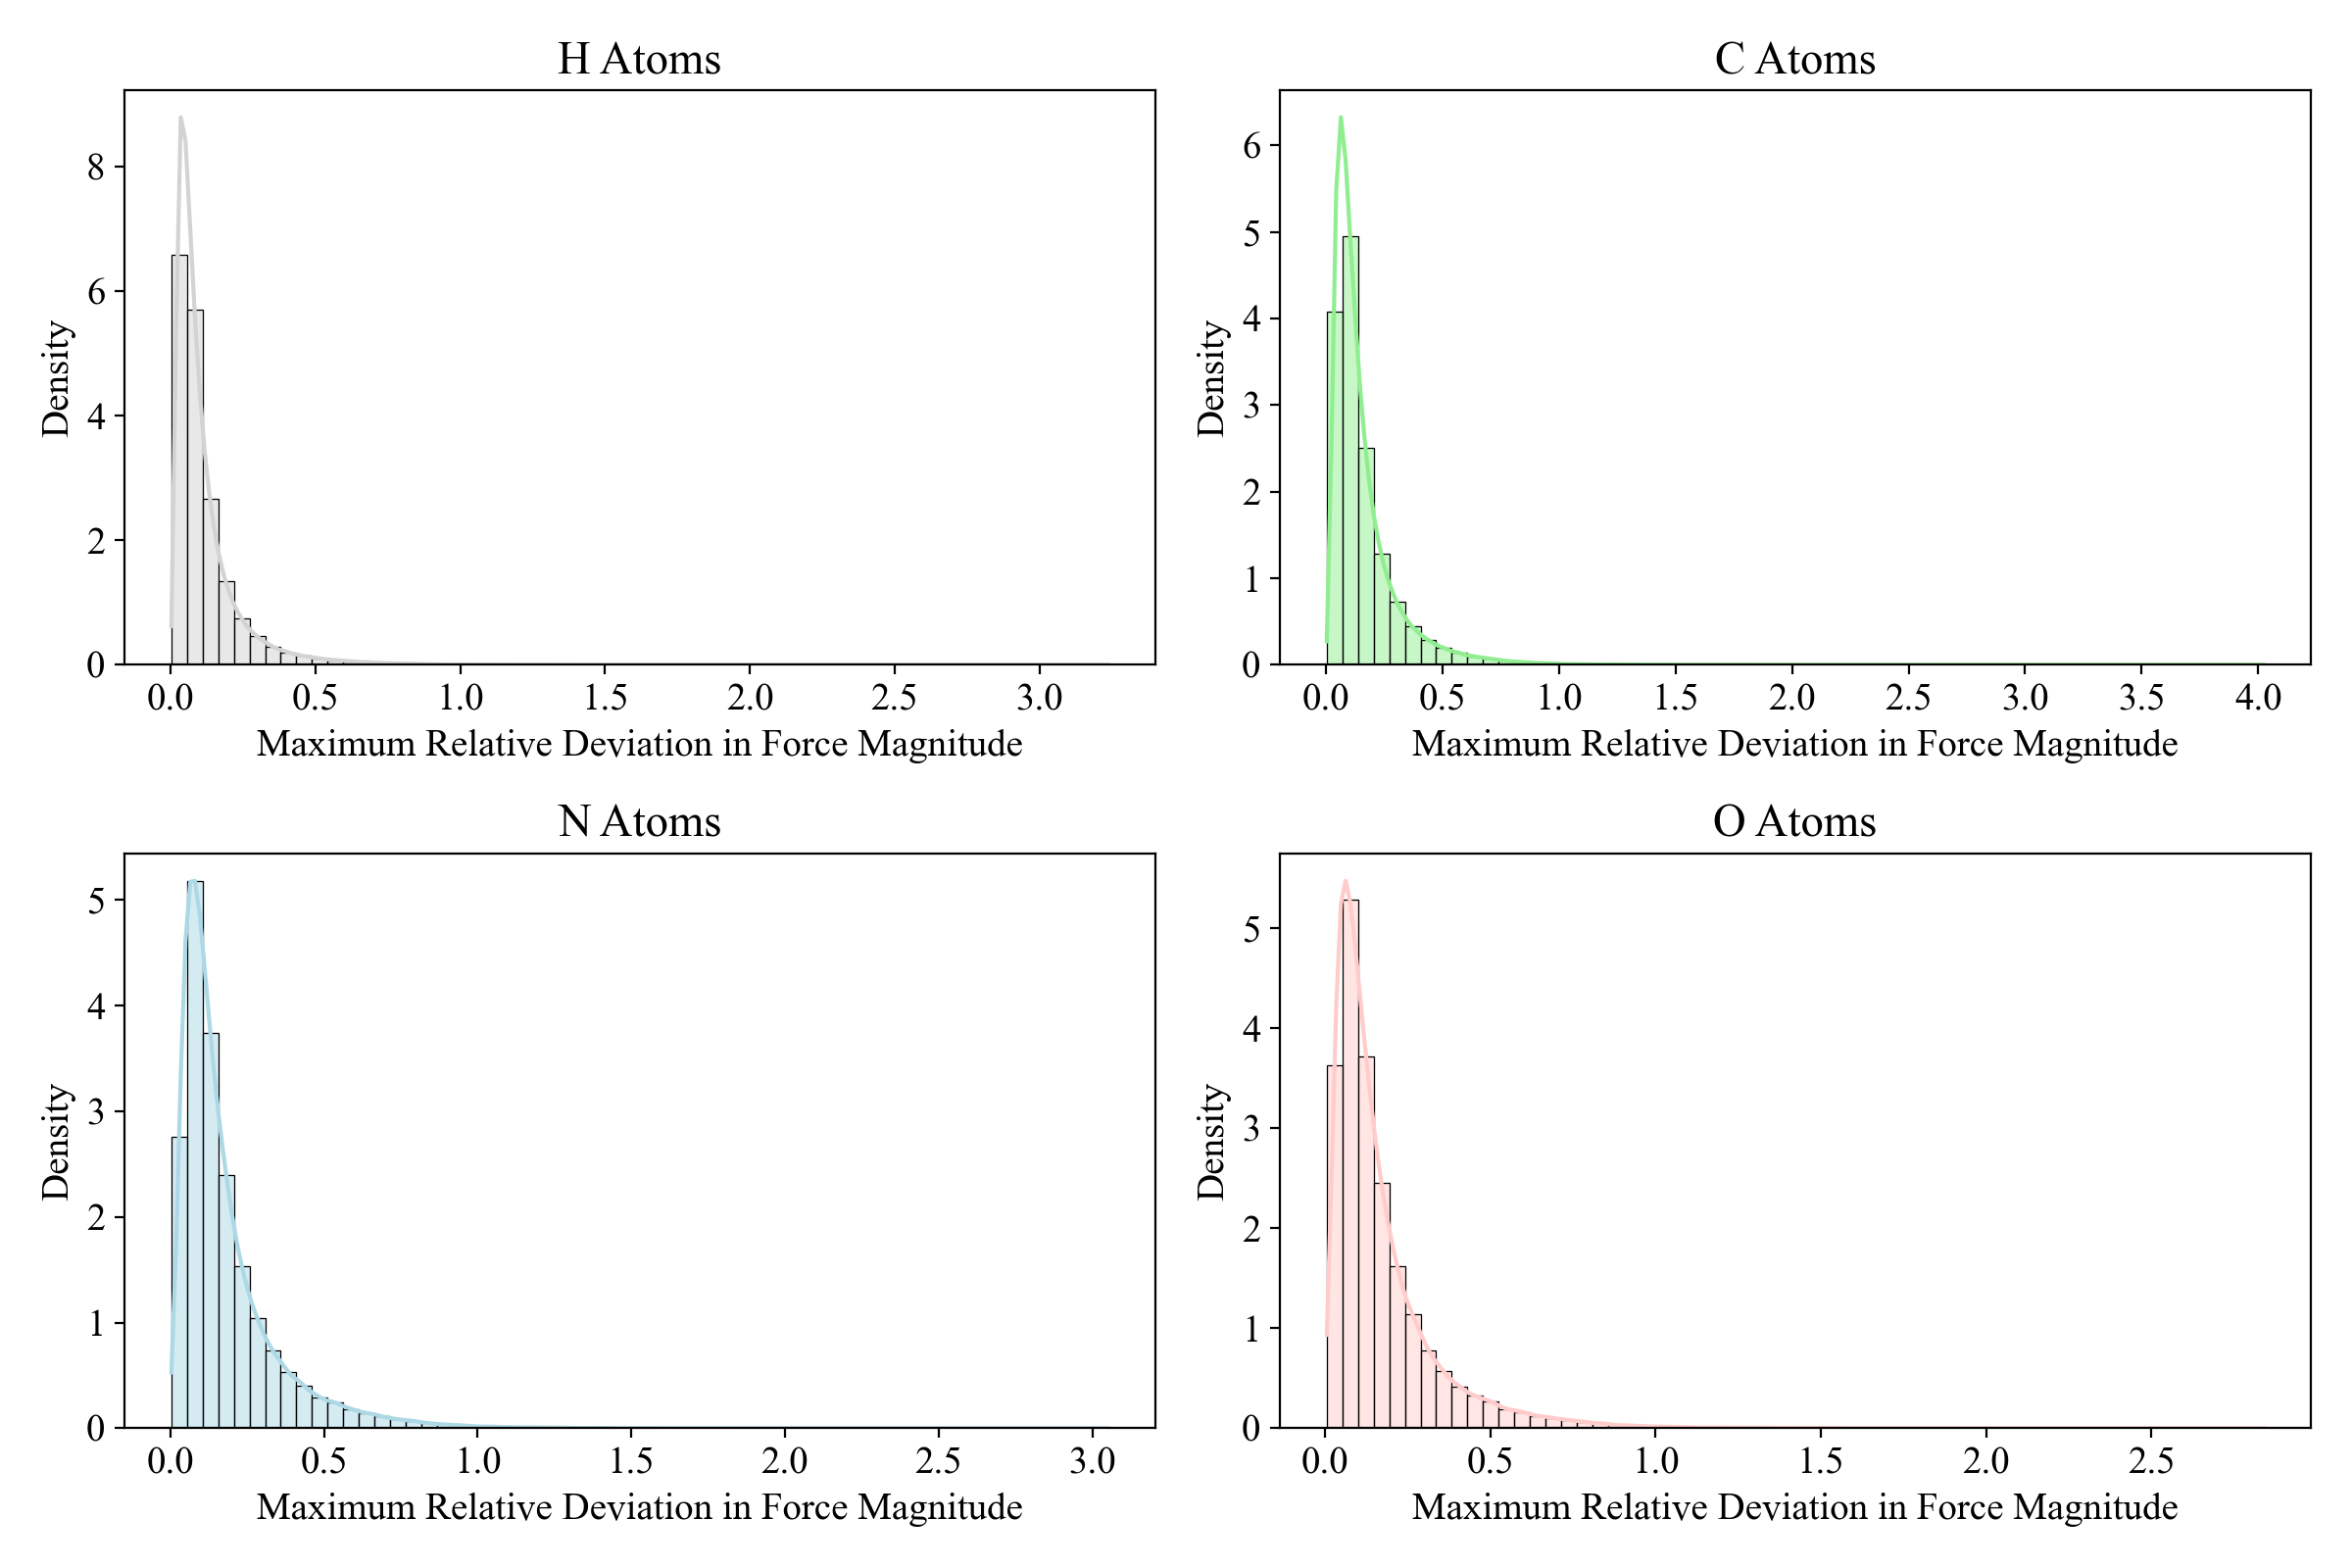
\includegraphics[width=0.9\linewidth]{Images/2xr_forces/max_force_deviation_by_species_subplots.png}
    \caption[Values of atomic deviation by atom type (COMP6v1)]{Values of atomic deviation by atom type across the COMP6v1 benchmark dataset ($N_\text{atoms}=$ 2,608,858). Values here are unitless, as they are normalized by the mean $|\vec{F}|$ prediction.}
    \label{fig:atomic_deviations}
\end{figure}

The distribution of \verb|atomic_deviation| values for each atom type are given in Figure \ref{fig:atomic_deviations} and the $N_\text{atoms}$ shown in each subplot in Figure \ref{fig:atomic_deviations} are given in in Table \ref{tbl:filtered_comp6v1_atom_count}.
It was empirically determined from the average value of \verb|atomic_deviation| in molecules with $\rho_{\vec{|F|}} \geq 3.5$, across the COMP6v1 benchmark dataset, that an \verb|atomic_deviation| $\geq 0.45$ selects highly uncertain atoms for any chemical species (H, C, N, O).

\begin{table}[h!]
\centering
\caption[Counts of each atom type in COMP6v1]{
Counts of each atom type in COMP6v1 used in the Figure \ref{fig:atomic_deviations} subplots.
}\label{tbl:comp6v1_atom_count}
\begin{tabularx}{0.26\textwidth}{lr}  
\toprule
Atom type & $N_\text{atoms}$ \\
\midrule
Hydrogen & 1,352,100 \\
Carbon & 890,691 \\ 
Nitrogen & 193,592 \\ 
Oxygen & 172,475 \\ 
Total & 2,608,858 \\
\bottomrule
\end{tabularx}
\end{table}

We then filtered for \verb|atomic_deviation| $\geq$ 0.45.
The filtered distribution of \verb|atomic_deviation| values is given in Figure \ref{fig:filtered_atomic_deviations}, and the $N_\text{atoms}$ shown in each subplot is provided in Table \ref{tbl:filtered_comp6v1_atom_count}.

\begin{figure}[!hb]
    \centering
    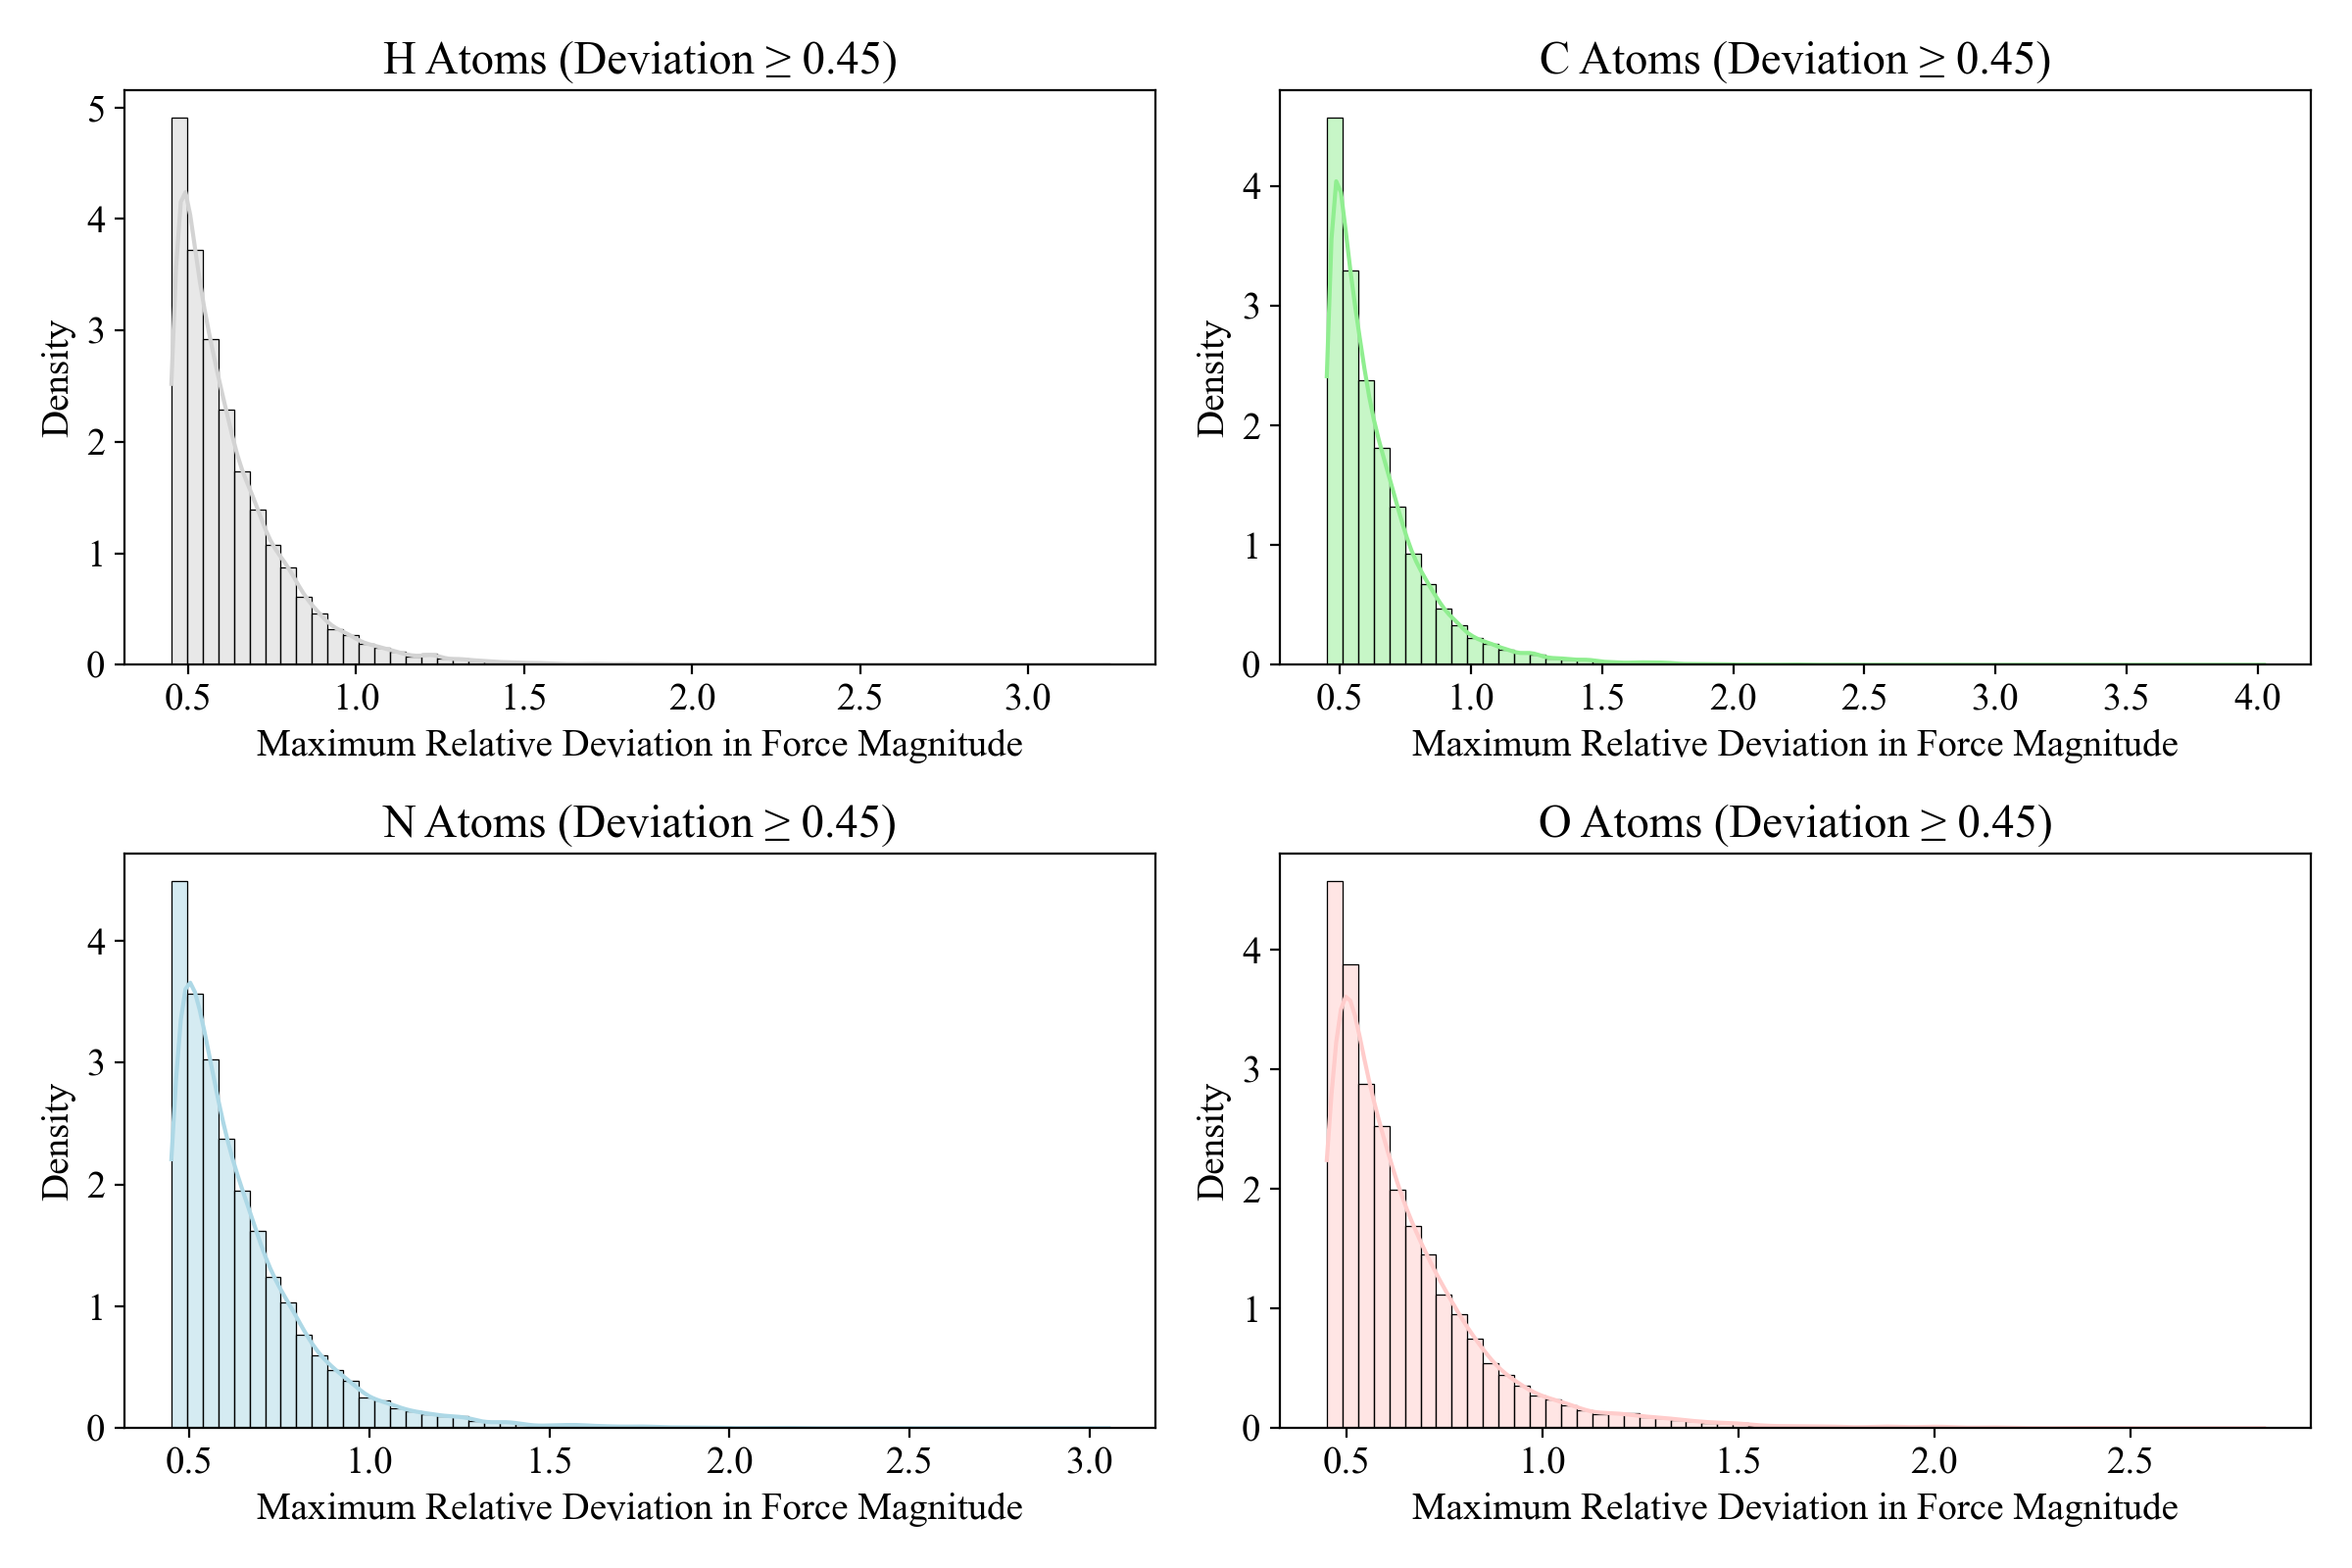
\includegraphics[width=0.9\linewidth]{Images/2xr_forces/max_force_deviation_by_species_filtered.png
    }
    \caption[Atomic deviation $\geq$ 0.45 by atom type (COMP6v1)]{Atomic deviation $\geq$ 0.45 by atom type across the COMP6v1 benchmark dataset ($N_\text{atoms}=$ 105,942). Values here are unitless, as they are normalized by the mean $|\vec{F}|$ prediction.}
    \label{fig:filtered_atomic_deviations}
\end{figure}

Note here that while hydrogen is by far the most prevalent element in the COMP6v1 dataset, a lower percentage of H atoms fall above an \verb|atomic_deviation| of 0.45 than the other atom types.
This is a good sign, because hydrogen atoms are very low mass relative to other elements and, due to the large number of these atoms, we sought a metric which does not bias toward the wider distribution of hydrogen force predictions.

\begin{table}[h!]
\centering
\caption[Counts of each atom type in the filtered COMP6v1]{
Counts of each atom type in the COMP6v1 benchmark dataset filtered for $\text{max deviation} \geq 3.5$, used in the Figure \ref{fig:filtered_atomic_deviations} subplots.
}\label{tbl:filtered_comp6v1_atom_count}
\begin{tabularx}{0.4275\textwidth}{lrr}  
\toprule
Atom type & $N_\text{atoms}$ & \% of COMP6v1 \\
\midrule
Hydrogen & 36,405 & 2.69\% \\
Carbon & 44,056 & 4.95\% \\
Nitrogen & 13,929 & 7.20\% \\
Oxygen & 11,552 & 6.70\% \\
Total & 105,942 & 4.06\% \\
\bottomrule
\end{tabularx}
\end{table}

Atoms marked with a high \verb|atomic_deviation| represent regions where the model is least confident in its force predictions and are therefore the most critical areas to improve.
Once these high-uncertainty atoms are identified, the next challenge is truncating the molecular environment in a way that preserves relevant chemical context. 
An example of the output from the first step in the LUKE pipeline is given in Figure \ref{fig:uncertain_atoms}, where there are two atoms (indices 2 and 11, colored magenta) marked for highly uncertain force predictions in the C\textsubscript{2}H\textsubscript{3}N\textsubscript{7}O\textsubscript{2} molecule.

\begin{flushleft}
\begin{multiFigure}
\begin{centering}
    \addFigure{0.4}{Images/atom_isolator/c2h3n7o2-cropped.png}
    \addFigure{0.4}{Images/atom_isolator/c2h3n7o2_highlighted-cropped.png}
\captionof{figure}[C\textsubscript{2}H\textsubscript{3}N\textsubscript{7}O\textsubscript{2}: High-uncertainty force magnitude predictions]{(A) C\textsubscript{2}H\textsubscript{3}N\textsubscript{7}O\textsubscript{2} molecule from ANI dataset; (B) highlighted atoms with a high atomic\_deviation value.
}
\label{fig:uncertain_atoms}
\end{centering}
\end{multiFigure}
\end{flushleft}

LUKE defines a tunable cutoff radius around each high-uncertainty atom, set to the AEV radial cutoff (5.1 $\angstrom$) in the initial release. 
Setting a cutoff radius to include only the nearest neighbors ensures that enough of the local atomic environment is retained to maintain chemically meaningful interactions, while avoiding unnecessary contributions from regions of the molecule with little interaction with the poorly predicted atoms. 
These extracted atomic environments are treated as independent molecular fragments, which can be computed at a reduced cost---relative to the whole-molecule they are extracted from---to be reintroduced into the training dataset.
By isolating and refining only the most uncertain atomic regions, this approach prioritizes data sampling where the model struggles most, rather than redundantly retraining on entire molecular structures with high energy uncertainty which contain many well-predicted regions.
A more focused data augmentation strategy has the potential to significantly reduce dataset size while maintaining or even improving predictive accuracy.

The process of isolating high-uncertainty atomic environments presents an opportunity to focus on reduced molecular representations that retain the key chemical patterns associated with high-uncertainty predictions. 
Instead of retraining ANI models on data containing large, computationally expensive structures, we can use these fragmented environments to identify simpler molecular motifs that capture the essential bonding interactions contributing to uncertainty. 
This approach aligns with broader trends in AI research within chemistry, where efforts to develop compressed molecular representations have led to advances in AI-driven drug discovery \cite{mol_reps_in_AI_drug_discovery_david} and systematic chemical pattern matching \cite{SMILES_pair_encoding_li, mol_patterns_SMARTS_schmidt, automated_fragment_gen_smiles_bilsland} through SMILES \cite{smiles} and SMARTS \cite{smarts} representations.
In the case of LUKE, the objective is to reduce molecular representations to the atomic environments which contain structural motifs that are poorly represented in the dataset-leading to highly uncertain prediction of energy and forces. 
A potential application of this method is in building a database of high-uncertainty small molecular representations, which could guide targeted data augmentation by focusing additional QM calculations on molecular substructures that ANI struggles to learn. 
As QM methods scale exponentially with the number of electrons in a system, this approach aims to significantly reduce the computational expense of generating new datasets for use in training future ANI models.
This does, however, present challenges in the data generation protocol utilized in active learning.

An example of the first approach to uncertainty-based molecular fragmentation of the molecule is given in Figure \ref{fig:uncertain_atoms}, where the two atoms from Figure \ref{fig:uncertain_atoms} (indices 2 and 11, colored magenta) with highly uncertain force predictions are isolated from the C\textsubscript{2}H\textsubscript{3}N\textsubscript{7}O\textsubscript{2} molecule.
By setting a cutoff radius with no other parameters, as can be seen in Figure \ref{fig:atom_isolator}, we slice through important parts of molecules, leaving behind unbonded atoms and improper valences.
Notice here that both of the structures produced have issues with chemical viability, with unbonded atoms or incomplete valences.
This shortcoming was present in every initial test in the early stages of LUKE development, and led to the consideration of additional processing to sanitize these fragments into real molecular structures. 

\begin{flushleft}
\begin{multiFigure}
\begin{centering}
    \addFigure{0.3}{Images/atom_isolator/c2h3n7o2_highlighted-cropped.png}
    \addFigure{0.3}{Images/atom_isolator/c2h3n7o2_11isolator-cropped.png}
    \addFigure{0.3}{Images/atom_isolator/c2h3n7o2_2isolator-cropped.png} \\
\captionof{figure}[Example output from the isolator stage of LUKE]{Example output from the isolator stage of LUKE on the (A)
C\textsubscript{2}H\textsubscript{3}N\textsubscript{7}O\textsubscript{2} dimer structure. Image (B) shows the truncation around atom 2 and (C) around atom 11. Note that the molecule is truncated at the AEV cutoff in either case; refer to Fig. \ref{fig:aev_radius} for an example of this cutoff radius.
}
\label{fig:atom_isolator}
\end{centering}
\end{multiFigure}
\end{flushleft}


One correction for this is to sanitize fragments using \verb|RDKit| \cite{rdkit}, which has algorithms check valencies, set aromaticity, conjugation and hybridization, and add hydrogen atoms where needed to ensure these conditions are met.
This approach to correcting unphysical structures presents additional challenges. 
First, there is a new computational expense in producing \verb|rdkit.mol| objects from the atomic species and coordinates used as inputs to ANI models.
For an individual object, this is not a slow process, but as a step in an active learning protocol, determining bonding configurations, generating SMILES strings, and sanitizing thousands molecules on-the-fly adds to the computational expense of generating new molecules for the training datasets before the data is even computed with QM.
This also requires precise handling and labeling of a large amount of data, especially in generating connectivities for dimer structures with \verb|RDKit| or \verb|OpenBabel| \cite{babel}.

More importantly, this implicitly alters the chemical environment to be represented, even if no new atoms are added within the AEV radius.
Hydrogen capping provides a straightforward way to satisfy valency constraints and maintain a chemically reasonable representation of the isolated substructure. 
However, this alters the AEV input representation that the ANI model originally learned from.
By truncating an aromatic ring, this approach introduces changes to symmetry and hybridization of orbitals, significantly altering the chemical behavior of boundary atoms.
While capping ensures that the fragment is a well-defined molecule, it may no longer resemble the high-uncertainty environment that necessitated its selection in the first place. 
Despite an awareness to these challenges, \verb|v0.1| of LUKE: Use the Forces incorporates a simple fragment sanitization scheme, and is set up to handle \verb|XYZ| and \verb|HDF5| file types for input and output. 
A sanitized example of the two molecules produced from the isolator stage of LUKE, shown in Figure \ref{fig:atom_isolator}, is given in Figure \ref{fig:sanitization}.

\begin{flushleft}
\begin{multiFigure}
\begin{centering}
    \addFigure{0.4}{Images/atom_isolator/cropped_atom11.png}
    \addFigure{0.4}{Images/atom_isolator/cropped_atom2.png}\\
\captionof{figure}[Sanitized output structures from LUKE]{
Sanitized structures from the  C\textsubscript{2}H\textsubscript{3}N\textsubscript{7}O\textsubscript{2} molecule. Image (A) shows the sanitized structure output from isolating the local chemical environment around atom 11 and (B) shows the sanitized molecule output from isolating around atom 2.
}
\label{fig:sanitization}
\end{centering}
\end{multiFigure}
\end{flushleft}

Notice here that the structure in (A) is exactly the same as in Figure \ref{fig:atom_isolator}, while (B) shows that the chemical environment around atom 2 has been reduced to a single fragment, losing the unbonded nitrogen and hydrogen atoms.
Without any additional logic to decide valences, \verb|RDKit| tries to retain the same as before---even when the \verb|AddHs| function is used.
In order to get sanitized structures, we convert the \verb|.xyz| file into a \verb|.mol| file with \verb|OpenBabel| \cite{babel} to get connectivity information, then load the \verb|mol| object into \verb|RDKit| and use the \verb|Sanitize| and \verb|GetMolFrags| functions to fill valences and filter out the nonbonded atoms, respectively.
Improving this process requires logic for neutralizing the molecules, which is complicated; the simplest solution is to drop atoms that have improper valences, but these are often found within a molecule that has been truncated around a high-uncertainty atom.
This is especially complicated when the atoms of concern are within a ring structure. 

Generating and packaging data into a format that is useful for training ANI models is vital to the utility of this process for applications in active learning.
In addition, LUKE contains functions to generate simple Gaussian \cite{gaussian16} input files and SLURM \cite{slurm} submission scripts for use in starting QM calculations as soon as highly uncertain chemical environments are detected.
LUKE represents a step toward precision-driven model refinement, where retraining efforts are concentrated on the most challenging chemical motifs rather than entire molecules. 
However, in the current state LUKE is not a catch-all approach to generating new data.
This protocol has no conformational sampling integrated and relies on external tools to manipulate molecular conformations.
Further, as with the sampling techniques used in generating the ANI-1x \cite{1x_1ccx_datasets} and 2x \cite{2x_dataset} datasets, this method entirely neglects configurational sampling, necessitating a more conscious approach to data generation.


\subsection{Drawback: Configurational Sampling}
\label{subsec:drawback_config_sampling}

While the LUKE approach offers a strategy for identifying and retraining on high-uncertainty atomic environments, it presents a fundamental limitation: the lack of diverse molecular configurations. 
By extracting and truncating molecular substructures, we improve the representation of high-error atomic environments in training data but do little to expand the broader diversity of molecular configurations that ANI encounters during inference. 
A fundamental distinction in molecular datasets is the difference between conformational and configurational diversity. 
Conformational sampling refers to generating different 3D structures of a given molecule, such as exploring torsional rotations around flexible bonds or sampling vibrational distortions near equilibrium geometries. While this form of sampling is important, it is inherently limited to a fixed set of configurations, meaning that it does not expand the diversity of molecular connectivity patterns available to the model.
Historically, ANI datasets—including ANI-1x \cite{1x_1ccx_datasets} and ANI-2x \cite{2x_dataset}—have relied heavily on conformational sampling to introduce new training data.
The molecules in these datasets were sourced from large enumerated molecular databases, such as GDB-13 \cite{gdb-13} and GDB-17 \cite{gdb-17}, which contain systematic lists of all possible stable organic molecules up to a given number of heavy atoms.
These datasets provide exhaustive coverage of stable molecules with up to 13 or 17 heavy atoms, respectively, ensuring that small organic structures are well-represented.

However, a major issue with this approach is dataset redundancy. 
The GDB databases were designed for small molecule discovery and drug-like compounds, meaning that a vast majority of the structures they contain exhibit similar functional groups and molecular motifs. 
The result is an oversampling of certain chemical environments, leading to a model that performs well on common molecular patterns but struggles when exposed to molecules that differ significantly from those in training. 
The consequence of this presents a hole in configurational diversity: the model lacks exposure to entirely new molecular architectures. 
If we only expand the training set through conformational sampling, we remain constrained to a narrow region of chemical space, improving accuracy within that limited domain but failing to generalize beyond it.
This means that ANI models will inevitably encounter molecules during inference that fall well outside their learned chemical space, leading to poor extrapolation and unreliable predictions for novel molecules.

To truly enhance ANI’s reliability, we need to go beyond conformational sampling and introduce configurational sampling—the process of systematically expanding the molecular connectivity space that the model has access to. 
While conformational sampling ensures that a given molecule’s low-energy geometries are well-represented, configurational sampling ensures that a model encounters diverse bonding topologies, functional group variations, and novel molecular frameworks.
A promising source of configurational diversity is ChEMBL \cite{ChEMBL_gaulton}, a large database of bioactive molecules with experimentally validated drug-like properties. 
Unlike GDB-derived datasets, which primarily contain small, stable organic molecules, ChEMBL includes a broader range of chemically relevant structures, including pharmacophores and complex heterocycles commonly found in medicinal chemistry, reactive intermediates and metabolites, which provide insights into chemical reactivity, and transition-state-like geometries, which are critical for understanding reaction dynamics. 
By incorporating ChEMBL-derived molecules into the training process, we can expand ANI’s knowledge of chemical space, enabling it to generalize more effectively to novel compounds.

Another approach to increasing configurational diversity is the systematic generation of new molecular fragments based on high-uncertainty atomic environments. 
As explored in the Subsection \ref{subsec:luke}, truncated high-uncertainty regions provide insight into molecular motifs that challenge ANI’s predictions. 
If we can map these motifs to larger molecular frameworks, we may be able to generate new molecules that share key bonding characteristics but provide fresh chemical contexts for model training.
This discussion leads to a critical consideration: If ANI models struggle most in specific atomic environments, should active learning strategies focus on fine-tuning the model using extracted high-error substructures, or should they instead prioritize generating novel configurations that explore previously unseen regions of chemical space? 
The LUKE approach stands to enhance model refinement, but it does not necessarily expand the configurational diversity of the training set.

A more balanced solution may involve a hybrid approach—using high-uncertainty atomic fragments as a guide for selecting new molecular configurations, allowing the model to learn from both localized uncertainty and broader molecular diversity. 
This concept is explored in greater depth in Section \ref{sec:exploring_new_mol_configs}, where we examine how configurational sampling methods can be used to improve the coverage of ANI-predicted potential energy surfaces.

\section{Outlook}

The exploration of uncertainty in ANI predictions has revealed both the strengths and limitations of current ensemble-based error estimation approaches.
While total molecular energy uncertainty, measured via query by committee (QBC), has been a useful heuristic for active learning, our investigation has shown that atomic forces provide a more resolute measure of uncertainty on the atomistic level.
By shifting the focus from total energy deviations to localized force-based uncertainty measures, we have outlined a potential pathway toward more targeted and data-efficient model training strategies.
The development of LUKE: Use the Forces provides a first step in refining active learning strategies, allowing us to focus training on high-uncertainty regions of molecular space rather than ensemble predictions of the global energy. 
However, as discussed in Section \ref{subsec:drawback_config_sampling}, this approach alone does not address the need for configurational diversity.

A significant challenge in this workflow is ensuring that the truncated molecular fragments remain chemically valid after removal from their original structure.
When an atom is extracted from a larger molecule, its local bonding environment is disrupted, potentially leading to unrealistic chemical representations.
To address this, we explored capping the truncated fragments with hydrogen atoms, a common strategy in force field parametrization and molecular fragmentation \cite{protein_ff_fragmentation_nn_wang}.
Direct chemical perception, such as the strategy proposed by Mobley et al. \cite{direct_chem_perception_mobley}, could further refine how we define chemically relevant fragments.
An integrated approach that combines uncertainty-driven substructure selection with configurational sampling strategies may offer the most efficient path toward improving model generalization.
By focusing on substructures that contribute most to model uncertainty, we can enhance predictive accuracy while minimizing computational cost. 
Future work should involve integrating pattern-recognition algorithms for detecting recurring uncertainty motifs, such as SMILES-based matching methods \cite{SMILES_pair_encoding_li} to identify chemically similar environments that may require additional training data. 

Beyond the refinement of existing training data, the uncertainty quantification methods explored in this work could also facilitate the expansion of ANI datasets to include additional elements, most notably phosphorus, which would enable the ML-driven simulation of RNA, DNA, and other complex biomolecular systems. 
Systematic detection of localized regions of high uncertainty provides a powerful tool for identifying failures in ANI predictions that could otherwise limit the applicability of large-scale simulations. 
The ability to capture, with QM-level accuracy, structural rearrangements in long-timescale simulations of complex biomolecules would significantly enhance large-scale biochemical modeling. 
Moreover, these improvements could extend to other reactive species that play critical roles in prebiotic chemistry---which is explored in Chapters \ref{chapter4} and \ref{chapter5}.
